\documentclass[10pt, a4paper]{article}

% Language setting
\usepackage{kotex}
% \renewcommand{\familydefault}{\sfdefault}
\usepackage[utf8]{inputenc}
\renewcommand{\figurename}{그림}
\renewcommand{\tablename}{표}
\renewcommand{\contentsname}{목차}
\renewcommand{\listfigurename}{그림 목차}
\renewcommand{\listtablename}{표 목차}
\renewcommand{\thesection}{\arabic{section}장}
\renewcommand{\thesubsection}{\arabic{section}.\arabic{subsection}}
\renewcommand{\thesubsubsection}{\arabic{section}.\arabic{subsection}.\arabic{subsubsection}}

% Page Size, Margins
\usepackage[a4paper,top=38mm,bottom=38mm,left=35mm,right=35mm,headheight=15mm, footskip=15mm]{geometry}

% Indentations
\setlength{\parindent}{2em}
\usepackage{indentfirst}

% Line Spacing
\usepackage{setspace}
\setstretch{1.6}

% Useful packages
\usepackage{amsmath}
\usepackage{graphicx}
\usepackage[colorlinks=true, allcolors=blue]{hyperref}
\usepackage{pgfplots}
\usepackage{float}
\pgfplotsset{compat=1.18}
\usepackage{makecell}
\usepackage{url}

% TOC Spacing (Fixes overlap between chapter numbers and titles)
\usepackage{tocloft}
\setlength{\cftsecnumwidth}{3em}
\setlength{\cftsubsecnumwidth}{3em}

% Path to figures
\graphicspath{{figures/}}

\title{영지식 증명 기반, 프라이버시를 보존하는 수치형 의료 데이터에 대한 증명 검색 시스템 \\ \bigskip \large Privacy-Preserving Proof Search System for Numerical Medical Data based on ZKP}
\author{황보진우 \and 박수용}
\date{\today}

\begin{document}
% \begin{titlepage}
%     \centering
%     \vspace*{2cm}
%     {\huge \bfseries 영지식 증명 기반, 프라이버시를 보존하는 \\ 수치형 의료 데이터에 대한 증명 검색 시스템 \par}
%     \vspace{1cm}
%     {\Large Privacy-Preserving Proof Search System for Numerical Medical Data based on ZKP \par}
%     \vfill
%     {\LARGE 2026년 7월 \par}
%     \vfill
%     {\LARGE 서강대학교 대학원 \par}
%     {\LARGE 컴 퓨 터 공 학과 \par}
%     {\LARGE 황 보 진 우 \par}
%     \vspace*{2cm}
% \end{titlepage}

% \begin{titlepage}
%     \centering
%     \vspace*{2cm}
%     {\huge \bfseries 영지식 증명 기반, 프라이버시를 보존하는 \\ 수치형 의료 데이터에 대한 증명 검색 시스템 \par}
%     \vspace{1cm}
%     {\Large Privacy-Preserving Proof Search System for Numerical Medical Data based on ZKP \par}
%     \vfill
%     {\LARGE 지도교수 박 수 용 \par}
%     \vfill
%     {\LARGE 이 논문을 공학석사 학위논문으로 제출함 \par}
%     \vfill
%     {\LARGE 2026년 7월 7일\par}
%     \vfill
%     {\LARGE 서강대학교 대학원 \par}
%     {\LARGE 컴 퓨 터 공 학 과 \par}
%     {\LARGE 황 보 진 우 \par}
%     \vspace*{2cm}
% \end{titlepage}

% \begin{titlepage}
%     \centering
%     \vspace*{2cm}
%     {\huge \bfseries \underbar{논 문 인 준 서} \par}
%     \vspace{1cm}
%     {\Large 황보진우의 공학석사 학위논문을 인준함 \par}
%     \vfill
%     {\LARGE 2026년 7월 7일\par}
%     \vfill
%     % \right
%     {\LARGE 주심 \space\space\space\space 박 \space\space 성 \space\space 용\par}
%     {\LARGE 부심 \space\space\space\space 박 \space\space 수 \space\space 용\par}
%     {\LARGE 부심 \space\space\space\space 최 \space\space 재 \space\space 승\par}
%     \vspace*{2cm}
% \end{titlepage}

\clearpage
\hypersetup{linkcolor=black}
\tableofcontents
\clearpage
\listoffigures
\clearpage
\listoftables
\clearpage
\hypersetup{linkcolor=blue}

%! TEX root = main.tex

\begin{center}
    {\huge \bfseries 감사의 글 \par}
\end{center}
\vspace{1.5cm}

이 논문이 완성되기까지 많은 도움과 격려를 아끼지 않으신 분들께 마음 깊이 감사의 인사를 전합니다. 
2년 전의 저는 컴퓨터 공학에 대한 기반 지식도 거의 없었으며, 무엇보다 연구란 어떤 것인지 전혀 알지 못하는 주니어 개발자였습니다.
하지만 박수용 교수님을 통한 좋은 기회로 이 분야의 전문성을 더할 기회를 얻었고, 석사 과정으로 학교로 돌아오게 되었습니다.
힘든 시간이었지만 많은 것을 배웠고 또 이러한 학문의 길이 저를 또다른 삶으로 인도할 것이라는 확신을 얻을 수 있었습니다.
비록 여전히 아는 것 보다 모르는 것이 훨씬 더 많지만, 저는 이것이 연구자로써의 첫걸음이라 생각합니다.
이 논문을 기점으로 저는 더 심오한 연구의 세계로 진입하고자 합니다.
향후 더 깊이있는 연구를 통해 연구자로서 세상에 많은 기여를 할 수 있는 큰 사람으로 거듭나도록 하겠습니다.
부족한 저를 끝까지 지도해 주신 박수용 교수님, 마지막에 완성도를 높일 수 있도록 도와주신 박성용, 최재승 교수님께 감사의 말씀 드립니다.

\clearpage


%! TEX root = main.tex

생성형 AI 서비스의 등장 이후로 전세계의 학계와 산업계가 모델을 학습할 대량의 데이터를 요구하기 시작하였다. 그렇게 다양한 분야에서 전에 없던 수준의 고품질 데이터에 대한 수요가 폭증하자, 데이터는 하나의 전략 자산과도 같은 위상을 지니게 되었다. 결과적으로 기존에 데이터를 독점하고 있던 각 분야의 플랫폼 기업들이 막강한 영향력을 떨칠 수 있게 되었지만 정작 데이터의 생성에 기여한 개인들은 아무런 보상도 받지 못한 채, 기업들의 신뢰할 수 없는 인프라에 의존하게 되는 상황이 지속되었다. Web 3.0은 이러한 데이터 자산 시대에 소유권 구조를 바로잡기 위한 비전으로 각광받기 시작했고, 많은 공학자들이 이를 위한 기술 개발에 몰두하였다. 특히나 많은 연구들이 데이터 원작자의 소유권을 보호하면서 자유롭고 안전하게 데이터를 거래할 수 있는 시스템을 구현하는 것을 목표로 이루어졌다. 본 연구는 그러한 시도의 일환으로써, 영지식 증명 기술을 이용해 데이터의 원문이 아닌, '증거'를 검색하는 시스템을 제안한다. 그 중에서도 수치로 표현되는 의료 데이터를 범위를 기반으로 검색할 수 있는 시스템을 제안함으로써, 환자 개개인이 자신의 의료 데이터가 유출될 걱정 없이 플랫폼에 증거를 업로드, 데이터 수요자는 이를 검색하여 필요한 범위에 적합한 데이터의 존재를 확인할 수 있게 한다. 이 시스템은 zk-SNARK 기반의 영지식 증명 데이터만을 중앙집중 서버에 저장하여 개인정보 유출의 위험을 제거하며, 동시에 수요자가 원하는 범위의 데이터를 효율적으로 검색할 수 있는 시스템을 제안한다.

\clearpage
\section{서론}
%! TEX root = main.tex

\subsection{연구 배경}

데이터는 산업과 학계에서 원자재와 같은 중요한 전략 자산이 되었으며, 특히 생성형 AI 서비스의 대중화를 계기로 고품질 데이터에 대한 수요가 폭증하고 있다. 그중에서도 의료 분야에서 생산되는 데이터는 개인의 생명 및 건강과 직결된 가장 민감한 정보로, 그 활용 가치만큼이나 매우 강력한 수준의 보안이 요구된다. 그러나 의료 데이터가 지닌 높은 가치는 곧바로 공격자들의 표적이 되고 있다. 최신 2025년 데이터 침해 비용 보고서에 따르면, 의료 산업은 14년 연속으로 전 세계에서 데이터 유출 피해 비용이 가장 높은 산업으로 기록되었으며, 침해로 인한 평균 비용은 무려 742만 달러(USD)에 달한다\cite{ibm2025cost}. 공격자들은 신분 도용이나 보험 사기 등의 금융 범죄를 목적으로 환자의 개인식별정보(PII)와 의료 기록을 집중적으로 노리고 있다. 더욱 치명적인 것은, 이러한 의료 데이터 침해 사고를 식별하고 통제하는 데 평균 279일이라는 긴 시간이 소요되어 타 산업 대비 피해 규모가 눈덩이처럼 커진다는 점이다.

\bigskip

이처럼 의료계에서 데이터 보안의 중요성이 갈수록 절실해지면서, 근본적인 보안 위협을 줄이기 위한 핵심 원칙으로 '데이터 최소화(Data Minimization)'가 대두되고 있다. 데이터 최소화란 시스템이나 서비스 제공에 반드시 필요한 데이터만을 수집 및 보관하고 그 외의 정보는 철저히 배제하는 것을 의미한다\cite{accessnow2021gdpr}. "수집되지 않은 데이터는 사람들에게 피해를 줄 수 없다"는 원칙 아래, 불필요한 데이터의 수집과 보존을 제한하는 것은 프라이버시 침해를 예방하고 시스템의 보안을 강화하는 가장 사용자 친화적이고 확실한 방법으로 평가받고 있다.

\bigskip

이러한 데이터 최소화 원칙을 시스템적으로 구현하면서도 데이터를 안전하게 유통하기 위해 최근 적극적으로 도입되고 있는 암호학적 기술이 바로 영지식 증명이다. 영지식 증명을 활용하면 개인의 건강 지표나 임상 기록과 같은 민감한 원본 데이터를 외부에 전혀 노출하지 않으면서도, 해당 데이터가 특정 조건을 만족한다는 사실만을 수학적으로 완벽하게 증명할 수 있다. 

\bigskip

\begin{figure}[ht]
    \centering
    \includegraphics[width=1\linewidth]{figure01.png}
    \caption{Gao et al. 외 많은 연구들이 제시한 데이터 증명 시스템의 일반적인 구조}
\end{figure}

하지만 의료 데이터 보안이나 검증 가능한 데이터베이스를 다룬 기존의 많은 연구들은 영지식 증명을 쿼리가 요청될 때마다 조건 일치 여부를 실시간으로 계산하고 버리는 '일시적인 증명 수단'으로만 사용해왔다. 그림 1은 Gao et al.이 제시하는 영지식 증명을 활용한 데이터 거래 시스템\cite{gao2024}의 아키텍쳐를 나타내고 있다. 이는 탈중앙화를 지향하는 데이터 거래 플랫폼 연구들이 대부분 차용하는 일반적인 구조이다. 이 구조에서 데이터 소유자는 데이터를 IPFS(Inter-Planetary File System) 등의 분산 파일 시스템에 저장하고, 해시를 블록체인에 저장하며, 스마트 컨트랙트를 통해 영지식 증명을 수행, 데이터를 재암호화 하여 수요자에게 제공한다. 이 과정에서 실시간 영지식 증명을 통해 소유자는 데이터의 특정 조건 만족 여부를 수요자에게 증명한다. 대부분의 아키텍쳐는 이처럼 데이터 수요가 발생할 때 마다 새로운 증명을 생성하고, 검증 후 폐기하는 구조를 가진다.

\bigskip

이러한 구조는 몇가지 한계를 지닌다. 우선 데이터를 IPFS와 같은 분산 파일 시스템에 암호화 하여 저장한다 하더라도, 결국 소유자가 아닌 제 3자의 시스템에 데이터를 위탁하는 셈이 된다. 이는 이들 연구가 지향하는 데이터 주권의 취지를 약화시키는 요소이다. 또한 스마트 컨트랙트를 통해 데이터 증명과 검증을 수행하는 과정은 소유자와 수요자 간의 1대1 통신으로 이루어진다. 이는 대량의 데이터를 요구하는 기업 및 기관 등에서 활용하는데 있어, 확장성의 문제를 야기한다. 이에 본 연구는 일회성으로 생성되고 버려지는 영지식 증명 데이터들을 한데 모아, 수요자들이 데이터의 존재 여부만 '검색' 할 수 있는, 따라서 오직 소유자의 단말기에만 데이터 원문을 남겨두는 안전한 '증명 검색 시스템(Proof Search System)'을 제안하고자 한다.

\subsection{문제 정의}

\textbf{데이터 프라이버시와 검색의 이중성:} 의료 데이터와 같은 민감한 개인정보를 거래하는 플랫폼이 상용화되기 위해서는, 수요자가 원하는 조건에 부합하는 데이터가 플랫폼 내에 얼마나 존재하는지 확인할 수 있는 '검색' 기능이 필수적이다. 동시에 민감한 정보인 만큼, 검색에 반드시 필요한 속성을 제외한 데이터의 다른 부분들은 철저히 숨겨져야 한다.

\bigskip

그러나 검색과 데이터 프라이버시는 본질적으로 상극의 이중성을 지닌다. 데이터의 유용성은 정보량이 높을수록 증가하지만 그만큼 프라이버시는 감소한다. 마찬가지로 검색의 성립을 위해선 데이터의 일부를 공개를 해야하지만, 그 순간 개인의 프라이버시는 침해될 수 있는 본질적인 모순이 발생한다. 결과적으로, "어떻게 하면 데이터의 원문 그 자체, 혹은 검색에 필수적이지 않은 부분을 은닉하여 데이터 최소화를 실현하면서도, 실시간 처리가 가능한 수준의 검색 효율성을 동시에 달성할 수 있는가?"가 본 연구가 해결하고자 하는 핵심 문제이다.

\subsection{연구 목적}

데이터 거래 플랫폼은 다양한 세부 프로세스들의 집합으로 이뤄진다. 플랫폼 내에서 데이터의 검증, 결제, 전달, 가공, 위탁 등 수많은 시나리오들이 유기적이고 무결하게 이뤄져야 한다. 본 연구는 그러한 시나리오 가운데 가장 첫 단계라 할 수 있는 '데이터 존재 여부의 확인', 즉 검색에 대한 솔루션을 제공한다. 그리고 이를 위해 다음과 같은 핵심 아이디어들을 활용한다.

\bigskip

\textbf{① 원문을 저장하지 않는 증명 검색 시스템:} 일반적인 검색 시스템과는 달리 본 연구는 데이터의 원문을 일절 저장하지 않는다. 대신 원문의 수치가 특정 범위 안에 존재한다는 범위 증명(ZKRP, Zero Knowledge Range Proof) 데이터를 저장하여 검색 대상으로 한다. 의료 영역에서 특정 수치가 일정 범위 안에 존재하는지의 여부는 중요한 진단 지표가 된다. 그리고 이러한 수치와 임계값 사이의 관계는 단순한 디지털 서명 등으로는 증명이 불가능하다. 여기서 영지식 증명을 활용하면 범위의 포함 여부를 확인하면서 동시에 정확한 수치를 공개하지 않는 것이 가능하다. 이를 통해 데이터 수요자는 원하는 데이터의 ‘신뢰 가능한 존재 여부’를 제공받고, 데이터 소유자는 원문의 유출에 대한 우려를 완벽히 제거할 수 있다.

\bigskip

\textbf{② 사전 정의된 참고치 기반의 오프라인 증명 생성:} 실시간 증명 생성의 병목을 해소하기 위해, 본 연구는 의료 데이터 도메인에 특화된 속성을 활용한다. 수치형 의료 데이터는 일반적으로 진단에 활용되는 절대적인 임상 참고치가 존재한다. 예를 들어, 세계보건기구(WHO) 가이드라인\cite{who2011}에 따르면 당화혈색소(HbA1c) 수치는 정상(5.7\% 미만), 당뇨 전 단계(5.7~6.4\%), 당뇨병(6.5\% 이상)으로 구간이 명확히 구분된다. 본 시스템은 이러한 사전 정의된 범위를 바탕으로 데이터 발급 시점에 영지식 증명을 미리 생성하여 서버에 저장한다. 이를 통해 검색 시점에는 실시간 회로 연산 없이 단순 DB 조회만으로 결과를 반환하여 검색 속도를 획기적으로 향상시킨다.

\bigskip

\textbf{③ 단일 그룹 커밋을 통한 복합 쿼리 소유권 증명:} 수요자가 복합 조건(예: 당화혈색소 6.5\% 이상 AND 공복혈당 126 이상)을 쿼리로 하여 검색할 때, 반환된 다수의 증명 데이터들이 모두 동일한 환자(소유자)의 것임을 보장해야 한다. 이는 ‘특정 환자가 어떤 데이터를 갖고 있는가’ 와 같은 환자에 대해 필수적이지 않은 추가 정보를 노출하는 문제를 발생시킨다. 본 연구는 이에 대한 해결책으로 개별 증명의 식별자들을 해싱하여 하나의 그룹으로 묶고(prf\_hash), 이를 소유자의 식별자(DP\_ID) 및 난수(nonce)와 결합하여 단일한 커밋을 생성한다. 이 방식을 통해 악의적인 공격자가 서로 다른 소유자의 데이터를 섞는 조작을 수학적으로 원천 차단하며, 그룹 내 증명 개수와 무관하게 단 1회의 증명 생성만으로 소유권을 입증하는 확장성을 달성한다.

\bigskip

이러한 접근을 통해 본 연구는 데이터 원문을 제 3자인 서버가 보유하지 않는 '완전한 영지식성'을 유지하면서도, 검색 조건에 부합하는 데이터의 존재를 증명할 수 있는 프라이버시와 검색 가능성 사이의 절충안을 제시한다. 이를 바탕으로 누구든 유출 걱정 없이 의료 데이터를 안전하게 판매 및 구매할 수 있는 신뢰도 높은 데이터 유통망 구축의 발판을 마련하고자 한다.

\clearpage
\section{관련 연구}
%! TEX root = main.tex

범위 데이터에 대한 안전한 검색 시스템은 데이터의 기밀성, 무결성, 그리고 검색 효율성 사이의 균형을 맞추기 위해 다양한 암호학적 기법과 시스템 구조를 통해 연구되어 왔다. 본 장에서는 기존 연구들을 주요 기술적 접근 방식에 따라 분류하고, 본 연구와의 차별성을 논한다.

\subsection{암호화 검색 및 순서 보존 암호}
초기 연구들은 암호화된 상태에서 데이터를 검색하기 위해 암호문의 순서를 평문의 순서와 동일하게 유지하는 순서 보존 암호(Order-Preserving Encryption, OPE)를 제안하였다. Agrawal et al. \cite{agrawal2004}은 수치 데이터에 대한 OPE 기법을 처음으로 제안하였으며, Shen et al. \cite{shen2021}은 이를 발전시켜 상태를 발생시키지 않는(Stateless) OPE 기법을 통해 아웃소싱된 데이터베이스에서의 범위 검색 효율성을 높였다. 또한, Popa et al.\cite{popa2011}이 제안한 CryptDB는 양파 암호화(Onion Encryption)라는 계층 구조를 통해 SQL 쿼리 유형에 따라 OPE나 결정론적 암호화(DET) 등 다양한 암호학 기술을 선택적으로 적용하여 실용적인 암호화 데이터베이스를 구현하였다. 

\bigskip

그러나 이러한 기법들은 암호문의 속성을 일부 노출한다는 본질적인 취약점이 존재한다. Naveed et al.\cite{naveed2015}은 OPE로 암호화된 데이터베이스에서 노출된 순서 및 빈도 정보를 바탕으로 원본 데이터가 복구될 수 있음을 증명하였다. 나아가 Islam et al.\cite{islam2012}은 일반적인 검색 가능 암호화 시스템에서도 노출되는 데이터 접근 패턴만으로 추론 공격을 통해 민감한 정보가 유출될 수 있음을 경고하였다. 본 연구는 이러한 보안 취약점들을 원천적으로 차단하기 위해 데이터의 순서나 접근 패턴을 포함해, 쿼리의 속성을 제외한 그 어떤 부가적인 정보도 노출하지 않는 영지식 증명(zk-SNARK)을 활용하며, 데이터 분포 노출을 막기 위해 사전 정의된 범위만을 증명하는 방식을 채택한다.

\subsection{공간 인덱스 및 비대칭 내적 연산 기반 검색}
앞선 순서 보존 암호의 데이터 순서 노출 문제를 방어하기 위해, 데이터의 평문 대소 관계를 숨기면서도 거리 비교를 가능하게 하는 특수 암호 연산과 공간 인덱스를 결합한 연구들이 등장하였다. 대표적으로 Wang et al.\cite{wang2013}은 다차원 범위 검색을 위해 R-tree의 최소 경계 사각형(MBR)을 비대칭 스칼라 내적 보존 암호(ASPE)로 암호화한 $\hat{R}$-tree를 제안하였다. 이 시스템은 쿼리와 데이터를 비대칭적으로 암호화하여, 서버가 원문을 모르는 상태에서도 내적 연산의 부호만으로 검색 범위 포함 여부를 판별할 수 있게 한다. 그러나 이 방식은 본 연구가 타겟하는 의료 데이터 검색 시스템에는 근본적으로 적용할 수 없는 치명적인 구조적 한계를 지닌다.

\bigskip

첫째, $\hat{R}$-tree의 MBR은 사용자가 임의로 지정하는 것이 아니라, 입력된 실제 데이터들의 최소값과 최대값을 둘러싸는 형태로 동적으로 결정된다. 반면 수치형 의료 데이터는 세계보건기구(WHO) 가이드라인과 같이 변하지 않는 '절대적인 임상 참고치'를 기준으로 진단과 검색이 이루어져야 하므로, 데이터의 분포에 따라 기준선이 매번 달라지는 동적 공간 인덱스 방식은 본 연구의 요구사항을 애초에 충족시킬 수 없다.

\bigskip

둘째, 순서 정보 은닉을 위해 데이터를 암호화된 노드 단위로 버킷화(Bucketization)하기 때문에, 쿼리 시 실제 조건에 맞지 않는 데이터까지 함께 반환되는 오탐(False Positives)이 필연적으로 발생한다. 의료 데이터 도메인에서는 미세한 수치 차이가 완전히 다른 임상적 진단을 의미하므로, 오탐을 허용하는 검색 모델은 의료 데이터 유통에 있어 가장 중요한 '결과의 신뢰성'을 상실하게 만든다. 이 밖에도 쿼리 처리를 위해 서버가 암호화된 인덱스를 순회하며 지속적으로 내적 연산을 수행해야 하는 연산 부담 역시 존재한다. 결론적으로, 동적인 범위 설정과 오탐을 수용하는 기존의 공간 인덱스 기반 검색은 정밀성이 요구되는 수치형 의료 데이터 도메인에 적용하기 부적합하다.

\bigskip

\subsection{동형 암호 및 학습형 인덱스 기반 검색}
공간 인덱스의 한계를 넘어, 데이터의 지역성을 기계학습으로 모델링하고 이에 동형 암호를 결합하여 프라이버시를 강화한 연구도 제안되었다. Wang et al.\cite{wang2025}이 제안한 SLRQ 시스템은 기계학습 기반의 학습형 인덱스를 구축하고, 이를 Paillier 가산 동형 암호로 암호화하여 아웃소싱하는 방식을 채택하였다. 이 시스템은 학습된 데이터 분포를 기반으로 후보군을 빠르게 탐색한 뒤, 오탐을 제거하기 위해 동형 암호화된 상태에서 개별 튜플과 쿼리 값을 정밀 비교하는 연산을 수행한다. 그러나 이와 같은 동형 암호 기반의 검색 방식은 실시간 시스템에 적용하기에 다음과 같은 몇가지 한계를 지닌다.

\bigskip

첫째, 동형 암호의 기하급수적인 연산 오버헤드로 인한 실시간성 훼손이다. 암호화된 상태에서 정밀한 대소 비교를 수행하기 위해서는 막대한 암호문 프로토콜(SIC, SM 등) 연산이 동반된다. 시스템의 보안성을 높이기 위해 암호화 키 길이를 증가시킬 경우 이러한 연산 지연은 기하급수적으로 증가하며, 결과적으로 단일 쿼리 처리에 수 초 이상의 시간이 소요되어 대규모 트래픽을 처리하는 실시간 검색 시스템에 부적합하다.

\bigskip

둘째, 복호화 권한의 존재로 인한 잠재적 정보 유출 위험성이다. SLRQ는 무거운 동형 암호 연산의 부하를 줄이기 위해 보조 연산 서버에 데이터베이스의 전체 비밀키를 제공하고, 난수가 섞인 형태이긴 하나, 데이터와 쿼리를 중간에 평문으로 복호화하여 비교하는 과정을 거친다. 이는 근본적으로 제3의 서버가 원문을 복원할 수 있는 권한과 수단을 갖게 됨을 의미하며, 해당 서버가 침해당하거나 노이즈 생성 패턴이 분석될 경우 의료 데이터의 기밀성이 치명적으로 유출될 수 있는 위험을 내포한다.

\bigskip

셋째, 동적 데이터 업데이트에 대한 취약성이다. 학습형 인덱스는 고정된 데이터 분포에 의존하기 때문에, 지속적으로 새로운 임상 데이터가 누적되는 의료 환경에서는 데이터 분포의 왜곡이 발생한다. 이를 해결하기 위해서는 정기적으로 전체 인덱스 모델을 재학습하고 다시 암호화하여 업로드해야 하는 막대한 유지보수 비용이 발생한다.

\subsection{검증 가능한 데이터베이스}
데이터의 기밀성 뿐만 아니라 쿼리 결과의 무결성을 보장하기 위한 연구들도 활발히 진행되었다. Zhang et al.\cite{zhang2015}의 IntegriDB와 vSQL은 아웃소싱된 데이터베이스에서 SQL 쿼리 결과가 정확하고 완전함(Sound \& Complete)을 암호학적으로 증명하는 시스템을 제안하였다. Li et al.\cite{li2023}의 ZKSQL은 이를 영지식 증명으로 확장하여 데이터 프라이버시를 강화하였다.

\bigskip

그러나 이러한 시스템들은 쿼리 시점에 실시간으로 증명을 생성해야 하므로 연산 오버헤드가 매우 크다. 특히 ZKSQL의 경우 일반적인 SQL 쿼리에 대해 수 초 내지는 수 분 이상의 증명 생성 시간이 소요되어, 실시간성이 요구되는 검색 서비스에 적용하기에는 한계가 있다. 본 연구는 이러한 실시간 증명 생성의 병목을 해소하기 위해, 데이터 업로드 시점에 '사전 정의된 범위'에 대한 증명을 미리 생성해 두고 검색 시에 이를 단순 조회하는 방식을 제안하여 검색 성능을 O(1) 수준(DB 조회 시간)으로 획기적으로 단축하였다.

\subsection{하드웨어 및 블록체인 기반 접근}
소프트웨어적 접근의 성능 한계를 극복하기 위해 신뢰 실행 환경(TEE)이나 블록체인을 활용하는 시도도 있었다. Zhou et al. \cite{zhou2021}의 VeriDB는 Intel SGX와 같은 신뢰 하드웨어 내에서 쿼리를 실행하여 무결성을 보장하며, Xu et al.\cite{xu2019}의 vChain은 블록체인 데이터베이스 상에서 누산기(Accumulator) 기반의 ADS(Authenticated Data Structure)를 통해 불리언 범위 쿼리의 무결성을 검증한다. 

\bigskip

하지만 하드웨어 기반 접근은 특정 제조사의 CPU에 의존해야 하고, 특정 연산이 특정 하드웨어에서 처리될 때 발생하는 여러 부산물(캐시 접근 패턴, 연산 소요 시간, 전력 소비량 , 전자기파 등)을 분석하여 진행되는 사이드 채널 공격(Side-channel Attack)의 위험이 있다. vChain과 같은 블록체인 기반 시스템은 데이터의 기밀성 보장보다는 무결성 검증에 초점이 맞춰져 있어 민감한 의료 데이터 보호에는 부족함이 있다. 본 연구는 특정 하드웨어에 의존하지 않고 범용적인 zk-SNARK 알고리즘만으로 기밀성과 무결성을 동시에 달성한다.

\bigskip

이처럼, 기존의 연구들은 검색 효율성을 위해 보안을 일부 희생하거나(OPE, CryptDB), 보안을 위해 효율성을 희생하는(ZKSQL, IntegriDB) 트레이드오프를 지니고 있다. 본 연구는 "zk-SNARK 기반의 사전 증명 생성"이라는 새로운 접근법을 통해, 데이터 원문과 순서 정보를 완벽히 은닉하면서도 실용적인 검색 속도를 보장하는 새로운 절충안을 제시한다. 그리고 동시에 현실의 데이터 수요를 고려해, 다중 쿼리의 처리에 대한 데이터 프라이버시와 소유권 증명을 모두 만족하는 방법론을 제시한다.


\clearpage
\section{배경 기술}
%! TEX root = main.tex

\subsection{zk-SNARK}
zk-SNARK(Succinct Non-interactive ARgument of Knowledge)는 범용 영지식 증명 기술 중 가장 대중적으로 널리 쓰이는 기술이다. 영지식 증명이란 어떠한 사실의 구체적인 내용은 밝히지 않으면서, 그것이 특정한 조건을 만족함을 수학적으로 증명하는 기술로, 데이터의 기밀성을 유지하면서도 무결성을 검증할 수 있게 한다. ‘범용(General-purpose)’ 영지식 증명이라 함은 특정 문제에 국한되지 않고, NP 복잡도 클래스에 속하는 모든 계산 문제를 증명할 수 있다는 의미이다.

\bigskip

zk-SNARK는 비 대화형 프로토콜(Non-interactive Protocol)의 일종이다. 이는 증명자와 검증자가 여러 번의 통신을 주고받아야 하는 대화형 프로토콜과 달리, 단 한 번의 증명 데이터 전송만으로 검증이 완료됨을 의미한다. 여기서 'Succinct(간결함)'는 증명 데이터의 크기가 매우 작고(수백 바이트 수준), 검증에 소요되는 시간이 증명하고자 하는 연산의 복잡도와 무관하게 거의 상수 시간(Constant time) 내에 이루어짐을 뜻한다.

\bigskip

zk-SNARK를 적용하기 위해서는 증명하고자 하는 연산(Computation)을 산술 회로(Arithmetic Circuit)의 형태로 표현해야 한다. 이 회로는 덧셈과 곱셈 게이트로 구성되며, 이는 다시 R1CS(Rank-1 Constraint System)라는 형태의 수학적 제약 조건 시스템으로 변환되어 처리된다. R1CS는 벡터의 내적 연산을 이용해 회로의 각 게이트가 올바르게 연산되었는지를 검증하는 방정식의 집합이다. 본 연구에서 활용하는 gnark 와 같은 프레임워크는 복잡한 R1CS 변환 과정을 추상화하여 제공함으로써, 개발자가 고수준의 코드로 회로를 정의할 수 있게 돕는다. 이러한 특성 덕분에 Zcash와 같은 블록체인에서의 트랜잭션 은닉 등 다양한 프라이버시 보호 시스템에서 핵심 기술로 활용되고 있다.

\subsection{Groth16 protocol}
Groth16 프로토콜은 현재 뛰어난 성능을 바탕으로 가장 널리 쓰이고 있는 zk-SNARK 프로토콜이다. 2016년 Jens Groth\cite{groth2016}가 처음 소개한 이 프로토콜은 증명 데이터의 크기와 검증 시간에 대해 상수 스케일의 복잡도를 달성하여 오늘날 zk-SNARK의 표준처럼 사용되고 있다. 본 연구 역시 해당 프로토콜을 기반으로 진행되었다.

\bigskip

증명자는 증명하고자 하는 선언(statement)을 다항식 세트 (Quadratic Arithmetic Program, QAP)로 표현한다. 예를 들어 증명자가 ‘$x^3+2x+7=19$를 만족하는 x값을 알고 있다’ 라는 사실(statement)를 x=2(witness)임을 밝히지 않으면서 증명을 한다면, 우선 x3+2x+7=19를 계산하는 과정을QAP라는 다항식 묶음의 형태로 치환해야 한다. 이 다항식들이 비밀 값(witness)을 내포하고 있는 다른 다항식으로 모두 나누어 떨어진다면, 검증자는 증명자가 옳은 비밀 값으로 그 QAP를 구성했다는 확신을 얻을 수 있다. 이 과정은 두 다항식이 하나의 임의로 선택된 점에서 교차한다면 충분히 높은 확률로 그 두 다항식이 동일하다는 Schwartz—Zippel Lemma에 의해 빠르고 효율적인 검증임이 증명된다. 그리고 암호화된 상태에서의 검증을 위해 이산로그 기반의 타원곡선 암호화 알고리즘, bilinear pairing등 여러 암호학적 장치들을 통해 이 검증 과정에서 증명 사실 외 다른 정보를 알 수 없도록 숨긴다.

\bigskip

Groth16은 비 대화형 프로토콜을 구현하기 위해 신뢰 셋업(trusted setup)이라는 공유 파라미터들을 증명 이전에 생성한다. 신뢰 셋업이란 검증자가 비밀의 내용을 모르고도 선언의 내용을 검증할 수 있게 하는 암호학적 파라미터들을 말한다. 대화형 프로토콜에선 증명자와 검증자가 서로 임의의 값들을 주고 받으며 처리해야 할 계산들을 이렇게 미리 합의된 값을 이용해 한번에 처리하는 방식이다. 검증자는 증명자가 제시한 다항식 위에서 임의의 한 점을 선택해 그에 대한 계산 결과를 검증해야 한다. 그런데 이 점이 증명자에게 노출되면 증명자는 해당 점을 포함하도록 다항식을 조작할 수 있다. 따라서 신뢰 셋업은 공개적인 과정을 통해 파라미터를 생성하여 그 임의의 점에 대해 서로 합의하는 과정이라고 볼 수 있다. 이 과정에서 Powers of Tau라 불리는 MPC(Multi-Party Computation) 프로토콜이 사용되며, 이는 참여자가 각자가 선택한 임의의 비밀 값 ��(tau)를 엔트로피로써 파라미터에 추가하는 과정으로 요약할 수 있다. 이 참여자 중 단 한명이라도 ��를 제대로 폐기했다면 이 신뢰 셋업의 기밀성은 수학적으로 보장되는 방식이다.

\subsection{Merkle Proof}
머클 트리(Merkle Tree)는 1979년 Ralph C. Merkle이 제안한 인증된 데이터 구조(Authenticated Data Structure, ADS)의 일종이다. 이는 대량의 데이터셋을 해시 함수를 이용해 이진 트리 형태로 요약한 구조로, 전체 데이터를 노출하지 않고도 특정 데이터가 해당 셋에 포함되어 있음을 효율적으로 증명(Membership Proof)하는 데 사용된다.

\bigskip

머클 트리의 핵심은 루트 노드(Merkle Root)가 트리 내의 모든 데이터에 대한 암호학적 압축값(Fingerprint) 역할을 한다는 점이다. 전체 데이터의 개수가 n일 때, 특정 리프 노드가 트리에 포함되어 있음을 증명하기 위해 전체 데이터를 검증할 필요 없이, 루트까지의 경로에 있는 해시값들(Sibling hashes)만 있으면 되므로 검증 복잡도는 O(log n)으로 매우 효율적이다.

\bigskip

본 연구는 이 머클 증명을 데이터 발급자(Data Issuer)의 유효성 검증에 활용한다. 시스템에 등록된 수많은 발급자의 공개키 중, 현재 데이터를 서명한 키가 유효한 목록에 포함되어 있다는 사실을 증명해야 한다. 이때 머클 증명을 zk-SNARK 회로 내부에서 수행함으로써, 검증자에게는 '유효한 발급자 중 한 명'이라는 사실만 알리고, 구체적으로 '누구'인지는 밝히지 않는 익명성을 보장한다. 이처럼 머클 증명은 블록체인의 트랜잭션 검증뿐만 아니라, 프라이버시를 보존하는 멤버십 증명 도구로서도 중요한 역할을 수행한다.

\subsection{zk-SNARK 친화적 암호화 원형 (zk-SNARK Friendly Cryptographic Primitives)}
zk-SNARK 시스템의 성능은 증명하고자 하는 연산을 산술 회로(Arithmetic Circuit)로 변환했을 때 생성되는 제약 조건(Constraints)의 수에 크게 의존한다. 일반적인 암호화 알고리즘(예: SHA-256, RSA)은 비트 연산이 많아 산술 회로로 구현 시 제약 조건의 수가 폭발적으로 증가하여 증명 생성 시간을 지연시킨다. 따라서 본 연구에서는 회로 내부에서의 연산 비용을 최소화하기 위해 대수적 구조가 간단한 zk-SNARK 친화적(zk-friendly) 암호화 원형들을 채택하여 사용한다.

\subsubsection{EdDSA (Edwards-curve Digital Signature Algorithm)} 
본 시스템은 데이터 발급자(DI)의 신원을 회로 내부에서 검증하기 위해 EdDSA 서명 알고리즘을 사용한다. EdDSA는 타원곡선 암호(ECC)의 일종으로, 특히 Twisted Edwards Curve 위에서 정의된다. 본 연구에서는 zk-SNARK 회로(주로 BN254 또는 BLS12-381 곡선 위에서 작동) 내부에 임베딩하기 적합한 Baby Jubjub 타원곡선을 사용한다. 이 곡선은 회로의 기본 필드(Base Field)와 호환되도록 설계되어 있어, 서명 검증 시 발생하는 타원곡선 덧셈 및 스칼라 곱셈 연산을 매우 적은 수의 제약 조건만으로 효율적으로 수행할 수 있다. 이는 수천 번의 곱셈이 필요한 RSA나 ECDSA에 비해 압도적인 성능 우위를 제공한다.

\subsubsection{MiMC (Minimal Multiplicative Complexity) Hash} 
데이터의 무결성을 검증하고 머클 트리(Merkle Tree)를 구성하기 위해 본 연구는 MiMC 해시 함수를 사용한다. 일반적으로 사용되는 SHA-256 해시 함수는 비트 단위의 논리 연산(XOR, Shift)을 다량으로 사용하므로 산술 회로 구현 시 수만 개의 제약 조건을 유발한다. 반면, MiMC는 유한체(Finite Field) 상에서의 세제곱 연산(x3)이나 역수 연산(x−1)과 같은 간단한 대수적 변환을 반복하는 구조로 설계되어 있다. 이러한 구조는 zk-SNARK의 산술 회로(R1CS) 표현에 최적화되어 있어, SHA-256 대비 수십 배 적은 제약 조건으로 동일한 보안 강도의 해시 연산을 수행할 수 있게 한다. 본 시스템의 머클 경로 검증(Merkle Path Verification) 로직은 MiMC를 사용하여 회로 깊이를 획기적으로 줄였다.

\subsubsection{암호학적 커밋 (Cryptographic Commitment)} 
데이터의 기밀성을 보장하면서도 특정 데이터가 변경되지 않았음을 증명하기 위해 암호학적 커밋 기법이 활용된다. 본 시스템에서는 다수의 검색된 증명 데이터들이 동일한 소유자(DP)의 것임을 영지식으로 증명하는 과정에서 정보를 노출하지 않기 위해 해시 함수 기반의 커밋을 사용한다. 특히 zk-SNARK 회로 내부에서의 연산 효율성을 극대화하기 위해 앞서 언급한 MiMC 해시 함수를 이용하여 소유자의 식별자(DP\_ID)와 증명 식별자들을 결합한 커밋을 생성하며, 이를 통해 완전한 은닉성(Hiding)과 위조 불가능성(Binding)을 달성한다.

\bigskip

이와 같이 본 연구는 회로 연산 비용에 최적화된 암호화 원형들을 전략적으로 선택 및 조합하여, 높은 보안성을 유지하면서도 실용적인 증명 생성 및 검증 속도를 달성한다.


\clearpage
\section{제안하는 시스템}
%! TEX root = main.tex

\subsection{구성 요소}

\begin{figure}[ht]
    \centering
    \includegraphics[width=1\linewidth]{figure02.png}
    \caption{System overview}
\end{figure}

본 연구는 영지식 증명 기반의 범위 데이터 검색 시스템을 제안한다. 이 시스템은 발급기관(DI), 데이터 소유자(DP), 데이터 수요자(DC), 검색 서버(SS)로 구성된 서로 다른 역할의 주체들을 포함한다. Figure 1은 본 시스템을 구성하고 있는 주체와 그들 간의 관계를 요약하고 있다. 발급기관이 데이터 소유자에게 데이터를 발급하고 데이터 소유자는 발급기관을 경유해 검색 서버에게 증명 데이터를 전달한다. 그리고 데이터 수요자가 증명에 대한 쿼리를 검색 서버에 전달하면 검색 서버는 그에 상응하는 증명의 목록을 수요자에게 반환하는 구조이다. 즉, 데이터 소유자가 증명을 서버에 제공, 데이터 수요자가 이를 검색하는 구조인 것이다.

\subsubsection{발급기관 (Data Issuer, DI)}
발급기관(DI) 은 사용자에게 데이터를 최초로 발급하는 주체로, 현실 세계에선 공공기관, 병원, 은행 등 인증된 개인정보를 보관하고 또 생성할 수 있는 주체들에 해당한다. 본 연구의 경우, 의료 데이터에 집중하기 때문에 병원 및 검진기관 등으로 고려할 수 있다. DI는 사용자에게 데이터를 발급하면서 본인의 비밀키로 서명을 생성하여 데이터에 첨부한다. 해당 비밀키에 대응되는 공개키는 검색서버(SS)의 데이터베이스에 저장된다. 

\subsubsection{데이터 소유자 (Data Provider, DP)}
데이터 소유자는 데이터에 대한 소유권을 지닌 주체로, DI 로부터 원본을 발급받는다. 현실에선 병원으로부터 의료 데이터를 발급받는 환자에 해당한다. DP는 DI로 부터 데이터를 발급받고 이를 디지털 지갑과 같은 개인화 된 저장소에 보관한다. 이 때, DI는 DP의 승인 하에 데이터를 검색 서버(SS) 에 전달할 수 있고, SS 는 전달받은 영지식 증명을 데이터베이스에 저장한다. 증명 생성 연산은 DI의 시스템에 위임하여 수행하며, DP의 단말기에서 직접 수행하는 것도 가능하다.

\subsubsection{데이터 수요자 (Data Consumer, DC)}
데이터 수요자는 DP의 데이터를 필요로 하는 주체로, 검색을 통해 원하는 속성에 해당하는 데이터를 찾고자 하는 쿼리의 주체이다. 현실에선 의료 데이터를 필요로 하는 제약회사 및 보험회사, 연구기관 등이 이에 해당한다. DC는 검색의 결과로 조회된 증명 데이터들을 로컬에서 직접 검증하여 찾고자 하는 데이터의 존재를 보장받을 수 있다.

\subsubsection{검색 서버 (Search Server, SS)}
검색 서버는 증명을 생성하는 역할과 쿼리를 처리하는 두가지 주된 역할을 맡는다. 우선 DP에게 데이터 원문을 전달받으면 이를 파라미터로 하여 증명 데이터를 생성한다. 생성된 증명 데이터는 검증키 및 메타데이터와 함께 데이터베이스에 저장되며 사용된 원문은 폐기된다. 그리고 DC로부터 속성과 범위를 포함한 쿼리를 수신하면, 그 속성과 범위에 해당하는, 증명 데이터 목록을 데이터베이스로부터 조회하여 반환한다. 

\subsubsection{데이터베이스}

\begin{figure}[ht]
    \centering
    \includegraphics[width=1\linewidth]{figure03-1.png}
    \includegraphics[width=1\linewidth]{figure03-2.png}
    \includegraphics[width=1\linewidth]{figure03-3.png}
    \caption{Database entity structure}
\end{figure}

SS는 검색 시스템을 구현하기 위해 세가지 엔티티 정보들을 데이터베이스에 저장한다. (1) PROOF의 경우, DI로부터 DP의 데이터를 전달받아 생성된 영지식 증명에 대한 정보들을 저장한다. 이는 쿼리의 대상이 되는 데이터이며 원문은 포함하지 않는다. (2) MERKLE의 경우, DI의 공개키로 구성된 머클 트리 정보를 저장하는 테이블이다. 이는 증명하고자 하는 데이터가 시스템에 등록된 DI에 의해 서명된 것인지 익명으로 확인하기 위해 필요한 데이터이다. (3) OWNERSHIP은 특정 PROOF 레코드가 어느 DP의 것인지를 나타내는 소유권 맵핑 정보이다. 해당 정보는 유출될 경우, 특정 사용자(DP)의 데이터 분포가 유추될 가능성이 있기 때문에, 분리된 내부 액세스 전용 데이터베이스로 관리된다. Figure 2는 SS와 연결된 데이터베이스가 가진 세개의 엔티티 구조를 나타내고 있다.

\subsection{데이터 발급 모델}

\begin{figure}[ht]
    \centering
    \includegraphics[width=0.8\linewidth]{figure04.png}
    \caption{Unit data structure}
\end{figure}

본 연구에서 다루는 데이터는 수치 데이터이므로 속성을 나타내는 정보(attribute)와 값을 나타내는 정보(value)가 필수적이다. 또한 의료 정보의 특성상, 기록의 발생 시간이 중요하므로 발급시간에 대한 정보(timestamp)도 필요하다. 그리고 이 세가지 데이터의 무결성을 검증하는 디지털 서명(signature) 역시 필요하다. 따라서 단위 데이터의 원문은 Figure 3와 같은 최소 형식을 따른다고 가정한다. 또한 데이터의 표현 형식은 가장 일반적인 표준인 JSON을 따른다고 가정한다.

\bigskip

예를 들어 ‘\{“attribute”: “attr0001”, “value”: 5.3, “timestamp”: 1768452114, “signature”: “3a8a98…2773aa”\}’와 같이 구성된 데이터가 있다고 가정하자. 그리고 “attr0001”은 “당화혈색소(HbA1c)” 를 참조하는 식별자라고 가정한다. 서명은 “attr0001" + "5.3" + "1768452114” 와 같이 나머지 정보들을 이어 붙여 구성된 메시지와 DI의 비밀키로 생성된다. 추후에 누구든 DI의 공개키를 이용해 이 서명을 검증할 수 있다. 실제로 발급되는 데이터는 이러한 단위 데이터들이 다수 모여 구성된 복합 구조체이며, DP가 가진 디지털 지갑과 같은 안전한 개인 공간에 저장된다.

\begin{figure}[ht]
    \centering
    \includegraphics[width=1\linewidth]{figure05.png}
    \caption{Data issue and proof generation process}
\end{figure}

\bigskip

증명 생성(proof\_gen) 프로세스의 시작에 앞서 ① DI는 DP에게 증명 생성에 대한 동의 여부를 묻는다. 이는 DI가 DP의 데이터를 위임하여 증명을 생성하기 때문이다. 물론 DP가 본인의 단말기에서 직접 증명을 생성해도 문제는 없다. 하지만 DP가 사용하는 단말기는 일반적으로 저사양의 모바일 기기이므로 수십, 수백개의 증명 데이터를 생성하는데 적합한 성능을 기대하기 힘들다. 따라서 데스크탑 및 워크스테이션의 연산능력을 활용할 수 있는 기관인 DI가 이 과정을 위임하는 것을 기본 시나리오로 상정하였다. ②, ③ DP는 자신의 개인키로 요청에 서명하여 이에 동의함을 표시한다. ④ DI는 DP의 데이터에 대해, 임상 참고치를 기반으로 범위 증명 데이터를 생성한다. 여기서 임상 참고치는 SS의 데이터베이스에 공개되어있으며, DI는 이를 불러와 사용한다. ⑤ 생성된 증명 데이터는 SS에게 전달된다. ⑥ SS는 요청을 수신하고 DP의 공개키로 서명을 검증한 후, ⑦ 데이터베이스에 증명 데이터들을 저장한다. Figure 4는 이러한 전체 과정을 도식화 하고 있으며, Figure 5는 DI에서 증명을 생성하고 SS에 전달하는 과정을 의사 코드로 나타내고 있다.

\bigskip

\begin{figure}[ht]
    \centering
    \includegraphics[width=0.8\linewidth]{figure06.png}
    \caption{DI side of proof generation process}
\end{figure}

여기서 미리 정의된 범위 구간은 각 항목이 참조하는 실제 의학적 참고치를 기반으로 한다. 예를 들어 세계보건기구(WHO)의 가이드라인\cite{who2011}에 따르면 당화혈색소의 정상 수치는 6.0\% 미만, 당뇨 전 주의 단계는 6.0 - 6.5\%, 당뇨 진단 기준이 6.5\% 이상이라고 한다. 이를 기준으로 하여 구간 정보를 (0, 6.0), (6.0, 6.5), (6.5, 100)와 같이 미리 정의할 수 있다. 앞서 언급한 사례의 경우, DP의 실제 데이터 수치가 5.3이라면 (0, 6.0)에 대한 범위 증명이 가능하다. 따라서 해당 범위 정보를 파라미터로 하여, 하나의 증명 데이터만 생성하게 될 것이다. 자세한 증명 생성 과정은 4.4에서 설명한다.

\bigskip

이와 같은 방식으로 모든 항목에 대해, 가능한 모든 범위 정보에 대해 증명 생성이 완료되면 이들은 모두 SS에게로 전달된다. 전달된 증명 데이터들은 PROOF 데이터베이스에 (항목, 범위 정보, 증명 데이터)의 단위로 정보를 저장하고, 또한 각 증명 데이터와 이를 제공한 DP의 맵핑 정보를 OWNERSHIP 데이터베이스에 저장한 후, 처리를 마친다.

\subsection{데이터 검색 모델}

\begin{figure}[ht]
    \centering
    \includegraphics[width=1\linewidth]{figure07.png}
    \caption{Proof search process}
\end{figure}

Figure 6는 데이터 검색 모델을 도식화 하고있다. 데이터 검색은 ① 데이터 수요자(DC)가 검색 쿼리를 검색 서버(SS)에 전달하면서 시작된다. 이 쿼리는 찾고자 하는 항목의 식별자(a)와 원하는 구간(r)을 포함한다. ② SS 는 PROOF 데이터베이스에서 쿼리의 항목과 구간에 해당하는 모든 증명 정보를 조회하여 ③ 반환한다. 이때 중요한 점은 증명의 소유자인 DP의 식별자(DP\_ID)는 결과에 포함되지 않는다는 것이다. 즉, 증명의 소유자에 대한 정보는 숨겨진다. DC가 알아야 할 정보는 자신의 쿼리를 만족하는 데이터가 분명히 존재한다는 증거 뿐, 이를 소유한 DP의 정체에 대해 알 필요가 없기 때문이다. Figure 2에서 PROOF 엔티티에 DP\_ID의 속성이 빠진 것은 이런 이유에서 이다. 다만 다중 쿼리의 경우, 다수의 증명에 대한 소유권 입증의 필요가 발생하기 때문에 이를 위한 별도의 OWNERSHIP 테이블을 데이터베이스에서 관리한다. 이에 대한 자세한 내용은 4.5에서 설명한다.

\bigskip

구간 정보는 쿼리에 담긴 구간 정보(r)가 단위 구간 크기보다 클 수 있다. SS는 이를 고려해 쿼리를 만족하는 모든 증명 데이터를 조회해야 한다. 예를 들어 DC가 당화혈색소가 위험구간 이상인 사람의 데이터를 검색하고자 한다면 (6.0, 100)과 같은 구간 정보를 쿼리로 전달할 수 있다. 이는 당뇨 주의 구간과 당뇨 진단 구간을 모두 포함하는 범위이다. 반면 SS의 데이터베이스는 (0, 6.0), (6.0, 6.5), (6.5, 100)의 3개 범위 정보를 취급하고 있다. 이때 SS는 (6.0, 6.5), (6.5, 100) 두개의 범위에 해당하는 PROOF 튜플들을 조회하여 반환해야 한다.

\bigskip

DC는 검색 결과로부터 증명 데이터를 다운받아 로컬 환경에서 zk-SNARK 검증 알고리즘을 수행해, 직접 증명을 검증할 수 있다. 검증에 필요한 컴파일된 회로 바이너리(R1CS) 데이터와 검증키 데이터는 SS에 공개되어있다. 증명 데이터는 데이터 원문이 해당하는 구간 안의 값을 가진다는 사실과 SS의 데이터베이스에 등록된 발급기관(DI)에 의해 서명되었다는 사실을 입증한다. 영지식 증명의 구체적인 구조는 4.4에서 설명한다.

\subsection{범위 증명 구조}

\begin{figure}[ht]
    \centering
    \includegraphics[width=1\linewidth]{figure08.png}
    \caption{Structure of range proof circuit}
\end{figure}

증명 생성 프로세스(proof\_gen)에서 만들어지는 증명($\pi$)은 Figure 7과 같은 구조의 회로(circuit)로부터 생성된다. 이러한 구조의 회로로 증명되는 사실은 (1) 데이터 원문 값이 특정 구간 안에 존재한다는 것과 (2) 데이터 원문에 첨부된 서명이 인증된 발급기관(DI) 의 공개키로 검증되었다는 사실, 두가지이다. 그리고 이 과정에서 DI의 정체를 숨기기 위해 DI의 공개키를 비밀 파라미터로 설정하는 대신, 머클 증명으로 해당 DI의 머클 트리 속 존재를 증명한다.

\bigskip

이를 위해 공개 파라미터로는 구간의 하단 값(range.lower)과 상단 값(range.upper), 데이터의 속성 정보(data.attribute)와 발급 시간(data.timestamp), DI 공개키로 구성된 머클 트리의 루트값(merkel\_root)이 할당된다. 이 정보들은 투명하게 공개되는 값이며, 추후 DC가 검증 시에 직접 확인하여 입력하는 항목들이다. 반면 비밀 파라미터로는 데이터 원문의 값(data.value), 발급 기관(DI)의 공개키(di.public\_key) 그리고 머클 증명에 사용될 머클 경로(merkle\_path)와 머클 비트(merkle\_bits)가 할당된다. 

\bigskip

회로 안에선 먼저 데이터가 주어진 범위의 하단 값과 상단 값의 사이에 존재하는지 확인하는 연산이 수행된다. 이 연산을 통과하면 데이터의 서명을 DI의 공개키로 검증하는 연산이 수행된다. 이 과정에서 사용되는 해시와 서명 알고리즘은 각각 zk-friendly 하다고 알려진 MiMC와 EdDSA를 사용한다. 여기까지의 연산은 데이터의 쿼리 만족 여부와 위변조 여부를 검사하는 계산이다. 다음으로 숨겨진 DI의 공개키가 시스템에 등록된 공개키의 집합에 포함된 것임을 증명하기 위한 머클 증명을 수행한다. 머클 증명은 리프 노드에 위치한 공개키에서 시작해, 주어진 머클 비트(왼쪽/오른쪽 정보)와 경로(형제 노드 정보)를 따라 루트 노드를 향해 점진적인 해시 계산을 수행한다. 최종적으로 계산된 값이 공개 파라미터로 주어진 루트 노드와 동일하다면 DI의 공개키는 머클 트리의 구성원임을 확인할 수 있다. 이렇게 특정 원소의 특정 데이터셋에 대한 포함 여부를 판단하는, 이른바 membership problem을 머클 증명을 통해 해결하면 시간 복잡도를 $O(N)$에서 $O(\log_2{N})$으로 줄이는 효과가 있다.

\bigskip

zk-SNARK 증명을 위해선 증명키와 검증키가 필요하고 이는 시스템 구축 시점에 진행되는 셋업(setup) 과정에서 미리 생성 되었으며, 누구나 공개적으로 접근할 수 있다고 가정한다. 이렇게 미리 생성된 키를 모든 증명/검증 과정에서 반복적으로 사용하는 것은 처리 속도를 높일 뿐 아니라, 악의적인 공격자가 조작된 키로 가짜 증명을 생성하는 것을 방지하는 효과가 있다. 또한 Groth16 프로토콜에서 셋업은 서킷의 구조에 종속되기 때문에 서로 다른 회로를 사용하는 증명들 사이에선 같은 키를 공유할 수 없다. 하지만 본 시스템의 범위 증명은 고정된 구조의 영지식 회로를 사용하기 때문에 단일 셋업을 통해 모든 증명 생성과 검증 작업을 수행할 수 있다.

\bigskip

다만 이러한 시스템을 현실에서 구현할 때는 추가적으로 고려해야 할 사항이 있다. 영지식 증명의 구조가 고정된 머클 트리를 가정하고 있기 때문이다. 머틀 트리는 시스템에 등록된 DI들의 공개키를 저장하는 자료구조이다. 따라서 새로운 DI가 추가되거나 삭제될 때, 혹은 키 유출로 인해 기존의 키를 무효화 하고 새로운 키를 등록해야 할 때 머클 트리의 구조는 지속적으로 변화한다. 이렇게 머클 트리의 구조가 변하면 기존 증명 데이터들의 유효성이 흔들리게 된다. 따라서 새로운 트리 정보가 추가될 때 마다, 상태 정보와 유효기간을 관리하여 새로운 증명과 기존 증명의 검증 유효성을 모두 보장하는 시스템이 필요하다. 또한 키 유출 등으로 더이상 증명의 무결성을 보장할 수 없게 된 경우, 해당 트리의 상태 정보는 폐기된 것으로 간주하며, 이를 통해 만들어진 증명 데이터도 폐기해야 한다. 본 연구는 이를 위해 SS가 관리하는 데이터베이스에 MERKLE 테이블을 추가하여 관리하고 있지만, 이러한 DI 머클 트리 정보에 대한 아카이브를 저장하는 데는 블록체인이 적합할 것으로 보인다. 블록체인은 수정할 수 없는 공개 데이터베이스와도 같기에, 증명의 무결성을 보장하기 위한 정보를 공시하기에 알맞은 수단이기 때문이다. 

\subsection{다중 쿼리의 처리}

다중 쿼리란 하나의 쿼리 안에 다수의 서브 쿼리(속성 – 범위 쌍)가 존재하는 경우를 말한다. 예를 들어 DC는 당뇨병 진단 환자의 데이터를 찾기 위해 당화혈색소가 6.5\% 이상인 동시에 공복혈당이 126 mg/dL이상인 환자의 증명을 검색하려고 할 수 있다. 이 경우 SS는 (당화혈색소 – (6.5, MAX)), (공복혈당 – (126, MAX))의 두 쿼리를 동시에 만족하는 DP의 증명들을 반환해야 한다. 그렇다면 검색 결과는 DP를 기준으로 그룹화된 증명의 목록의 형태를 가질 것이다. 하지만 4.3에서 설명한 것과 같이 DP\_ID는 숨겨지기 때문에 DC는 DP에 대한 그 어떠한 정보도 검색 결과에서 얻을 수 없다. 이로 인해 DC는 그룹으로 묶인 두 범위 증명(당화혈색소와 공복혈당)이 정말로 같은 DP로부터 생성된 것인지에 대한 확신이 필요하다. 악의적인 SS라면 전혀 다른 두 DP의 증명을 제시하며 DC를 기만할 수 있기 때문이다. 이처럼 다중 쿼리를 처리할 때는 '소유권 증명의 문제'가 발생한다.

\begin{figure}[ht]
    \centering
    \includegraphics[width=1\linewidth]{figure09.png}
    \caption{Process of composite query handling}
\end{figure}

\begin{figure}[ht]
    \centering
    \includegraphics[width=1\linewidth]{figure10.png}
    \caption{Commitment for ownership proof}
\end{figure}

이 문제를 해결하기 위해 다시 zk-SNARK 증명이 사용된다. ① 우선 DC가 다중 쿼리를 SS에 전달할 때, 고정된 크기의 임의의 바이트 값인nonce를 함께 전달한다. ② SS는 전달받은 다중 쿼리를 처리하기 위해 데이터베이스에서 PROOF와 OWNERSHIP 테이블을 JOIN 한다. 이렇게 JOIN된 테이블은 DP\_ID 정보를 가지게 된다. 여기서 DC의 쿼리로 필터링 한 튜플들을 DP\_ID를 기준으로 분류한다. ③ 그렇게 튜플들이 DP\_ID로 그룹화 되면, DP\_ID를 숨기기 위한 커밋(commitment)을 계산한다. Figure 9은 이 커밋을 계산하는 과정을 나타내고 있다. 한 그룹에 총 n개의 증명이 존재한다고 할 때, 이 n개 증명들의 식별자 값을 모두 더하여 해시한다(prf\_hash). 그리고 이 해시 값을 DP\_ID, nonce와 더한 후 다시 해시 한다. 이렇게 그룹의 모든 증명에 대한 식별자와 소유자(DP)의 식별자 정보를 함축한 커밋을 계산하되, DC가 제공한 임의의 값(nonce)를 추가하여 이를 랜덤화 하는 것이다. 커밋이 계산되면 튜플들을 분류하고 있던 DP\_ID를 커밋으로 대체한다. ④ 그리고 해당 커밋이 올바르게 계산되었음을 증명하는 영지식 증명을 생성한다. ⑤ 그렇게 커밋과 소유권 증명으로 묶인 범위 증명 항목들은 최종적으로 DC에게 검색 결과로써 반환된다. Figure 8은 다중 쿼리의 처리 과정을 나타내고 있다.

\subsection{소유권 증명 문제}

소유권 증명 문제는 다중 쿼리의 결과로 반환된 임의의 범위 증명 정보들이 동일한 DP\_ID와 연계되어 있음을 증명하는 문제이다. 본 연구는 이를 검색 서버(SS)가 다중 쿼리 결과를 그룹화하고 커밋을 계산할 때, 이 연산이 올바르게 수행되었음을 zk-SNARK를 통해 영지식으로 증명하는 방식으로 해결한다. Figure 10은 여기서 사용되는 산술 회로의 구조를  도식화 하였다.

\begin{figure}[ht]
    \centering
    \includegraphics[width=1 \linewidth]{figure11.png}
    \caption{Structure of ownership proof circuit}
\end{figure}

증명하고자 하는 DP\_ID의 커밋을 $c$, 증명의 식별자들을 ($p_1, \cdots, p_n$) 라고 한다. 공개 파라미터로 $c$와 ($p_1, \cdots, p_n$), 그리고 DC가  쿼리에 포함했던 nonce를 할당한다. 그리고 숨겨야 할 값인 DP\_ID는 비밀 파라미터로 할당한다. 산술 회로는 커밋을 계산하고 이를 파라미터로 주어진 $c$와 비교하는 연산을 수행한다. 두 값이 같을 경우, 결과로 반환된 커밋($c$)은 올바르게 계산된 것임이 증명된다. 참고로 여기서 사용되는 증명키와 검증키 역시 4.4에서의 증명과 마찬가지로 시스템 구축 초기에 진행된 셋업 과정을 통해 미리 생성되었으며, 공개된 것으로 가정한다. 증명이 생성되면 SS는 이를 DC에게 반환하며, DC는 이를 검증하여 커밋이 올바르게 계산되었음을 확인할 수 있다. Figure 11은 이와 같은 과정을 거쳐 최종 생성된 검색 결과 아이템의 한 예시를 보여주고 있다. 실제 검색 결과에는 이와 같은 데이터 구조체가 페이지 크기로 설정된 숫자 이하로 반환된다.

\begin{figure}[ht]
    \centering
    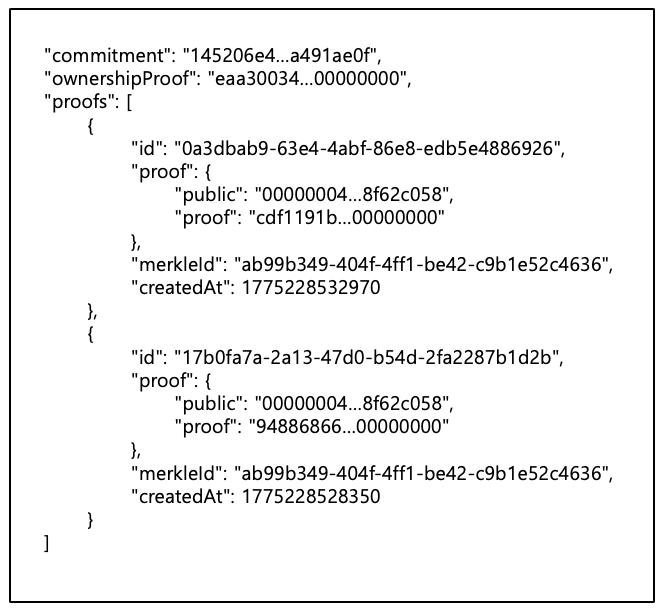
\includegraphics[width=1 \linewidth]{Figure12.png}
    \caption{Example of a single item in a composite query result}
\end{figure}

\subsubsection{소유권 증명 프로세스 최적화 (On-the-fly Batch Proof)}

다중 쿼리를 처리할 때, 실시간으로 소유권 증명을 생성하는 것은 일반적인 구현이라 볼 수 없다. zk-SNARK는 증명 생성의 연산 부담이 큰 기술이기 때문이다. 따라서 SS의 연산 부담을 줄이기 위해 쿼리 결과엔 커밋만을 포함하고 추후 DC의 요구에 따라(on-demand) 증명을 선별적으로 생성하는 것이 더 효율적일 수 있다. 하지만 본 시스템의 소유권 증명 회로는 MiMC와 같은 zk-friendly 해시 연산 위주로 구성된 경량 회로이므로, 수 밀리초(ms) 이내에 증명 생성이 가능하다. 따라서 클라이언트(DC)의 추가적인 요청을 기다리는 대화형(interactive) 방식 대신, SS가 검색 결과를 반환할 때 소유권 증명을 실시간으로 일괄 생성하여 동봉하는 비대화형(non-interactive) 방식으로 최적화하여 통신 지연을 최소화한다. 결과적으로 한 번의 쿼리 요청 및 응답(1 round-trip)만으로 검색과 소유권 검증이 모두 완료되므로, 시스템은 높은 실시간성을 확보할 수 있다.

\subsection{시스템 성능 및 보안성에 대한 고찰}
본 제안 시스템은 기존 연구들과 비교하여 확장성과 실용성 측면에서 다음과 같은 차별점 및 트레이드 오프(Trade-off)를 가진다.

\bigskip

첫째, 압도적인 확장성(Scalability)의 확보이다. 본 시스템의 증명 생성 비용은 전체 데이터베이스 크기(N)가 아닌, 검색 조건을 만족하여 필터링된 결과 그룹의 개수(K)에 선형적으로 비례(O(K))한다. ZKSQL\cite{li2023}과 같은 기존 연구들이 전체 데이터 세트에 대해 O(N) 이상의 다항식 연산을 수행해야 했던 것에 비해 이는 엄청난 성능적 이점이다. 더욱이 각 DP 그룹에 대한 증명 생성은 서로 완전히 독립적이므로, SS 환경에서 병렬 처리를 적용하면 다수의 DP에 대한 소유권 증명 비용을 쉽게 극복하고 대규모 시스템에 적용할 수 있다.

\bigskip

둘째, 실용성과 무결성 간의 현실적인 트레이드 오프이다. 본 시스템에서 증명의 근간이 되는 DP\_ID는 OWNERSHIP이라는 서버 내부의 비공개 데이터베이스에 존재한다. DC 입장에서는 SS가 이 테이블을 조회할 때 정직하게, 모든 튜플을 누락 없이 조회했는지 완벽하게 알 방법은 없다. IntegriDB\cite{zhang2015}나 ZKSQL\cite{li2023} 등의 검증 가능한 데이터베이스 기술을 적용하면 쿼리 결과의 누락이 없음(Completeness)을 수학적으로 보장할 수 있지만, 이는 쿼리당 수 분 이상의 증명 시간을 요구하여 '실시간 검색 서비스'라는 본 연구의 핵심 목적을 훼손한다. 물론 소유권 맵핑과 같은 민감 정보를 데이터베이스에 저장하는 것은 분명한 보안 취약점이다. 이에 대한 구체적인 내용은 5장 실험에서 밝히며, 대응 전략도 간략하게 소개할 것이다.

\bigskip

따라서 본 연구는 SS를 '결과를 임의로 누락할 수는 있지만(Incomplete), 없는 결과를 위조하거나 서로 다른 소유자의 데이터를 섞을 수는 없는(Sound)' 반신뢰(Semi-honest) 주체로 가정하였다. 이를 통해 프라이버시와 위조 불가능성이라는 핵심 보안 요건을 완벽히 달성하면서도 프로토콜을 실시간 처리가 가능할 만큼 경량화 할 수 있었다. 비공개 데이터베이스(OWNERSHIP) 조회의 완전한 무결성까지 실시간 수준으로 보장하는 방법론은 향후 연구 과제로 남긴다.

\clearpage
\section{실험}
%! TEX root = main.tex

본 연구는 영지식 증명을 사전 정의된 범위에 적용한 최초의 검색 시스템이므로, 직접적으로 비교할 수 있는 동일한 기능의 선행 연구가 존재하지 않는다. 따라서 본 장에서는 시스템의 실효성을 입증하기 위해 벤치마크 실험과 데이터의 원문을 저장하여 실시간으로 증명을 생성하는 baseline 모델을 구현하고 처리 시간과 용량 부담을 비교 측정하는 실험을 진행한다. 이로써 본 연구가 제시하는 '사전 생성된 증명에 대한 검색 시스템'의 효율성과 의의, 그리고 한계(trade-off) 등을 종합적으로 분석한다.

\subsection{실험 설계}

\subsubsection{마이크로 벤치마크}
우선 본 연구에서 사용하는 두가지 영지식 증명: 범위 증명과 소유권 증명에 대한 각각의 처리 시간을 측정한다. 한 속성 데이터에 대해 범위 증명을 생성하는데 소요되는 평균 시간과 다수의 데이터에 대한 소유권 증명을 생성하는데 소요되는 평균 시간을 측정한다. 범위 증명의 경우, 시스템에 등록된 DI의 수에 따라 회로의 크기가 달라지므로 이를 128, 256, 512, 1024로 지수적으로 증가시키며 시간을 측정한다. 소유권 증명의 경우, 처리하고자 하는 서브 쿼리의 수가 고정되어 있지 않으므로 최소 2개부터 시작하여 최대 5개까지 선형적으로 늘렸을 때 추가 소요되는 시간을 확인한다. 이렇게 시스템 성능의 핵심 요소인 영지식 증명의 처리 시간을 측정하여, 대규모 시스템에 적용하였을 시, 어느 정도까지의 부하를 감당해야 하는지를 예측할 수 있다.

\bigskip

또한 범위 증명과 소유권 증명에 대해 증명 데이터의 평균 크기도 함께 측정한다. Groth16 프로토콜의 특성상, 회로의 구조나 규모에 관계없이 증명 데이터의 크기는 항상 일정할 것으로 예상되며, 이를 확인할 것이다. 또한 데이터 원문은 단순 정수로, 4~8바이트 정도로 크기가 작은데 비해, 증명 데이터 바이너리는 크기가 상대적으로 크기 때문에 어느 정도의 용량 부하가 추가되는지 확인할 필요가 있다. 사전에 생성하여 저장하는 범위 증명 데이터의 크기는 시스템의 스토리지 부하에 영향을 끼치며, 실시간으로 생성되는 소유권 증명 데이터의 크기는 네트워크 부하에 영향을 끼칠 것이다.

\bigskip

마지막으로 실제 시스템에서 다중 쿼리를 처리하는데 소요된 시간을 상세히 측정할 것이다. 빈 응답이 없도록 구성한 다중 쿼리 100개를 한 세트로 하여, 서브 쿼리의 숫자를 2에서 5로 늘려가며 응답 시간을 측정한다. 이를 통해 실제 검색 시스템에서 사용자가 기다려야 하는 시간과, 전체 응답 시간 중 실시간 영지식 증명이 차지하는 비율을 확인할 것이다. 이를 통해 소유권 증명을 위한 실시간 증명의 트레이드 오프가 충분히 수용할 만한 수준이라는 것을 증명할 것이다.

\subsubsection{설계 방식 비교 실험}
본 연구가 제안하는 시스템의 가장 큰 특징은 사전 정의된 범위(pre-defined range)를 기반으로 증명 데이터를 발급 시점에 미리 생성하고, 검색 시점에 이를 조회하는 방식이다. 이로써 데이터 원문은 보유하지 않으면서 그것의 존재를 효율적으로 확인하는 것이 가능하다. 하지만 현실의 대부분의 검색 시스템은 데이터 원문을 보관하고 쿼리에 따라 원문의 속성을 직접 조회하는 방식으로 동작한다. 이같이 데이터 원문을 제 3자인 검색 서버가 보유하는 것은 시스템의 보안을 크게 훼손하는 일이나, 대부분의 경우, 이처럼 고객의 동의 하에 각종 개인정보를 위탁 관리하고 있다. 따라서 baseline 모델을 다음과 같이 정의하고, 본 연구가 제안하는 '사전에 생성된 증명 검색' 방식의 성능을 비교하였다.

\begin{itemize}
  \item 실시간 증명(on-the-fly ZKP): 데이터 원문을 데이터베이스에 저장한 후, 쿼리의 범위를 만족하는 튜플들을 조회하여 해당 튜플에 대한 범위 증명을 실시간(on-the-fly)으로 생성하여 반환하는 시스템.
  \item 측정 지표: 평균 쿼리 응답 시간. 정해진 100개의 쿼리에 대해 결과를 반환하기 까지의 시간을 측정하여 그에 대한 평균을 계산.
  \item 기대 결과: baseline은 조회되는 데이터의 수(페이지 크기)에 따라 수 초 이상이 소요될 수 있지만 제안 시스템은 밀리초(ms) 단위로 즉시 응답함을 보여 실용성을 입증.
\end{itemize}

또한 baseline 모델을 설계할 때, 원문을 암호화 하였을 때와, 하지 않았을 경우를 별도로 비교한다. 이는 성능을 우선하여 구현한 경우와 보안을 우선하여 구현한 경우를 제안된 모델과 함께 비교하기 위함이다. 원문을 암호화 할 경우, 쿼리 처리 과정에서 복호화 과정이 추가되며, 이는 곧 추가적인 성능 하락이 있을 수 있음을 암시한다. 암호 알고리즘은 AES-CTR을 채택한다. AES 알고리즘은 블록 기반 암호화 알고리즘으로, 블록 스킴(CBC, GCM 등)을 선택해야 하는데, 이 경우 CTR 스킴을 선택하였다. 이는 암호화 하는 데이터가 최대 64비트의 정수(수치형 데이터이므로)인데, CBC나 GCM과 같은 대중적인 블록 스킴을 사용하면 64비트의 용량 제한을 넘어서기 때문이다. 데이터 원문을 문자열의 형태로 저장하는 방법도 있지만 이는 불필요한 형변환 과정을 발생시키므로 처리 속도에 영향을 미친다. 반면 CTR 스킴은 스트림 암호화 스킴으로, 원문과 암호문의 크기가 동일하다. 따라서 실험의 환경에서 최적의 속도를 기대할 수 있다.

\bigskip

실험은 100만개($N = 10^6$) 데이터 셋을 임의로 생성하여 진행한다. 먼저 정해진 1000명의 DP 정보와 30개 속성 정보를 기반으로 100만 개의 데이터를 무작위로 생성하여 base 데이터베이스를 구성한다. 그리고 이를 기반으로 다시 서로 다른 DI 숫자(128, 256, 512, 1024)를 가진 각각의 환경에 대응하는 최종 데이터베이스를 생성한다. 이를 통해 발급자 정보만 다를 뿐, 데이터의 분포는 완전히 동일한 4개의 테스트 셋이 구성된다. 이 base 데이터베이스는 baseline 모델 뿐만 아니라, 제안 모델에서도 동일하게 활용되어, 총 12개의 동일한 분포를 지닌 테스트 셋이 만들어진다. 이로써 서로 다른 테스트 셋들이 DI 정보를 제외, 완벽히 동일한 데이터를 기반으로 구성되도록 한다.

\bigskip

실험은 다음 두 파라미터를 변경해가며 진행한다. 

\begin{itemize}
    \item \textbf{DI 수:} 시스템에 등록된 발급자(DI)의 수에 따라 범위 증명의 영지식 회로의 규모가 달라진다. 따라서 DI수를 달리 했을 때, 어느 정도로 부하가 증가하는지 측정하고 확장성을 판단한다. 실험에선 128, 256, 512, 1024의 DI를 사용한다.
    \item \textbf{페이지 크기:} 모든 검색 시스템은 처리 시간과 네트워크 부하 등의 이유로 기본적으로 페이징 시스템을 차용한다. 즉, 한번에 반환하는 페이지의 크기에 따라 응답시간도 변화할 수 밖에 없다. 따라서 페이지 크기를 점진적으로 늘렸을 때 어느 정도의 처리 지연이 발생하는지 측정하고 확장성을 판단한다. 기본 페이지 크기를 30으로 설정하였고 이를 60, 90, 120으로 늘리며 처리 시간을 비교 측정한다.
\end{itemize}

마지막으로 실험 환경에서 baseline 모델과 제안 모델이 사용한 데이터베이스와 각종 파일들의 용량을 비교할 것이다. baseline 모델은 정수형의 원문 데이터를 데이터베이스의 일부로 보관하지만 본 연구의 시스템은 원문 대신 증명 데이터를 별도의 바이너리 파일로 보관하기 때문에 어느정도 스토리지 부담이 증가할 수 밖에 없다. 따라서 실험 환경의 100만개 데이터가 만들어내는 스토리지 부하를 서로 다른 DI의 수에 따라 각각 측정하여 비교한다.

\subsubsection{위협 모델 시뮬레이션 및 확장 보안에 대한 고찰}

본 제안 시스템은 소유권 증명 쿼리 처리의 실시간성을 확보하기 위해, 검색 서버(SS) 내부에 민감 데이터인 OWNERSHIP 맵핑 테이블을 유지하는 반신뢰(Semi-honest) 위협 모델을 기본으로 설계되었다. 그렇기에 검색 서버가 외부 공격자나 악의적인 관리자에 의해 완전히 장악되어 OWNERSHIP 테이블을 포함한 모든 데이터베이스가 유출되는 최악의 시나리오를 가정할 경우, 프라이버시 침해 위협이 발생할 수 있다. 따라서 공격자의 입장에서 OWNERSHIP 데이터베이스를 장악했을 경우를 가정하여 취득한 데이터를 분석하고 시각화하는 시뮬레이션을 진행한다. 나아가 이러한 위협을 완화하기 위해 고려 가능한 전략을 함께 간략히 소개한다.

\subsection{실험 환경}

본 실험은 macOS를 구동하며, 애플 M4 프로세서, 16GB 통합 메모리, 256GB SSD 저장 공간을 지닌 Apple Mac Mini 환경에서 진행하였다. 실험에 사용된 모든 시스템 컴포넌트는 Go 언어(v1.25.1)로 작성되어 동일한 로컬 머신 상에서 구동되었으며, 측정된 시간 지표들은 네트워크 통신 지연을 배제한 순수 시스템 연산 시간을 기준으로 한다. 영지식 증명 프레임워크로는 gnark(v0.14.0)를 사용하였고, 회로 최적화를 위해 BN254 타원곡선과 MiMC 해시, EdDSA 서명 알고리즘을 적용하였다. 데이터베이스는 SQLite(v1.6.0)를, ORM 라이브러리로는 gorm(v1.31.1)을 사용하였다.

\bigskip

실험에 사용한 데이터는 총 1,000,000건($10^6$) 규모로, 모두 임의로 생성하여 앞서 언급한 base 데이터베이스를 구성하였다. 이는 본 시스템에서 다루는 데이터의 형태가 단일 수치로, 다른 데이터와 상호 관계성이 전무하므로 문제가 없다는 판단에 기반하였다. 생성된 수치 값들은 각 항목의 특성을 반영하여 주어진 범위 내에서 균등 분포(Uniform Distribution)를 가지도록 난수로 생성되었다. 데이터 속성 정보의 경우 실제 의료 데이터 거래 시나리오를 재현하기 위해 서울아산병원 건강정보 \cite{asan2014}를 참고하여 '당화혈색소', '공복혈당' 등 30개의 검진 데이터 항목을 수기로 작성하여 적용하였다. DP 정보는 1000개의 비대칭키 쌍을 생성하여 사용하였고 DI 정보는 각각 128, 256, 512, 1024개의 비대칭키 쌍을 생성하여 사용하였다.

\subsection{실험 결과}

\subsubsection{마이크로 벤치마크}

\begin{table}[h]
    \footnotesize
    \centering
    \begin{tabular}{p{3cm}|c|c|c|c}
        \hline
        DI Count & 128 & 256 & 512 & 1024 \\
        \hline
        Proof Gen Time(ms) & 75 & 80 & 83 & 86 \\
        Proof Size(Bytes) & 164 & 164 & 164 & 164 \\
        \hline
    \end{tabular}
    \caption{range proof benchmark}
\end{table}

\begin{table}[h]
    \footnotesize
    \centering
    \begin{tabular}{p{3cm}|c|c|c|c}
        \hline
        Sub-query Count& 2 & 3 & 4 & 5 \\
        \hline
        Proof Gen Time(ms) & 10 & 11 & 12 & 16 \\
        Proof Size(Bytes) & 164 & 164 & 164 & 164 \\
        \hline
    \end{tabular}
    \caption{ownership proof benchmark}
\end{table}

마이크로 벤치마크 실험에선 범위 증명과 소유권 증명에 대한 증명 생성 시간과 크기을 각각 측정하였다. 이를 통해 다음 세가지 사실을 입증할 수 있었다.

\bigskip

첫째, 범위 증명의 경우 시스템에 등록된 데이터 발급자(DI)의 수가 128개에서 1024개로 8배 증가함에 따라 증명 생성 시간은 75ms에서 86ms로 단 11ms(약 15\%) 증가하는 데 그쳤다. 이는 영지식 회로 내부에서 수행되는 발급자 공개키에 대한 머클 증명 연산이 $O(\log{N})$의 시간 복잡도를 가지기 때문이다. 즉, 발급 기관의 수가 대규모로 확장되더라도 개별 증명 생성 시간에 미치는 영향이 매우 미미함을 입증한다. 이를 통해 본 시스템의 확장성은 시스템에 등록되는 발급자의 수에 큰 영향을 받지 않음을 예측할 수 있다.

\bigskip

둘째, 다중 쿼리 처리를 위한 소유권 증명의 경우, 서브 쿼리의 개수가 2개에서 5개로 늘어날 때, 증명 생성 시간은 9ms에서 16ms로 소폭 증가하였다. 서브 쿼리의 개수가 증가할수록 개별 증명들의 식별자를 해싱하여 prf\_hash를 구하는 연산량이 늘어나지만, 최대 5개의 복합 조건을 처리할 때조차 절대적인 증명 생성 시간이 16ms로 매우 가볍다. 이 결과는 본 연구의 4.6.1절에서 제안한 소유권 증명에 대한 '실시간 일괄 생성' 최적화의 타당성을 뒷받침한다. 즉, 다중 쿼리에 대한 소유권 증명을 검색 서버(SS)가 쿼리 시점에 실시간으로 생성하더라도, 서버 연산에 미치는 부담이 극히 적어 높은 실시간성을 확보할 수 있음을 보여준다.

\bigskip

셋째, 파라미터나 회로의 구조에 관계 없이 모든 경우의 증명 데이터 크기가 일정하다. 이는 zk-SNARK의 특장점으로, 증명 대상의 속성에 관계없이 늘 일정한 크기의 증명 데이터가 보장된다. 이는 시스템을 확장했을 때 요구되는 스토리지 오버헤드를 쉽게 예측할 수 있게 해준다. 실제로 실험을 위해 생성한 $10^6$개 데이터에 대해 생성된 증명 데이터는 약 630 메가바이트로 측정되었다. 이는 검증의 편의성을 위해 공개 파라미터를 증명 데이터와 함께 저장하였기에, 나온 수치이다. 공개 파라미터를 제외하고 순수히 증명 데이터만 저장한다면 이를 약 164 메가바이트로 줄일 수 있다. 또한 페이지 크기가 30일 때 다중 쿼리에 대한 응답으로 반환되는 소유권 증명 크기의 총합은 164 $\times$ 30 = 4,920 바이트, 약 4.9 킬로바이트에 해당한다. 이는 일반적인 저해상도 이미지 한장, 혹은 그 이하에 해당하는 수준이기에 네트워크 부담을 크게 증가시키지 않는다. 이와 같이 zk-SNARK(Groth16)의 증명 데이터는 충분히 크기가 작으며 또한 고정되어있기에 대량의 데이터에 대해서도 용량 부담을 일으키지 않으며, 확장에 대한 리소스 예측을 용이하게 한다.

\bigskip

\begin{table}[h]
    \centering
    \footnotesize
    \begin{tabular}{l|c|c|c|c}
        \hline
        Sub-query Count & 2 & 3 & 4 & 5 \\
        \hline
        Overall & 3,711 & 5,340 & 7,156 & 9,019 \\
        DB Fetch & 3,253 & 4,878 & 6,696 & 8,556 \\
        Proof Gen & 454 & 458 & 457 & 459 \\
        \hline
    \end{tabular}
    \caption{average query response time(ms) for different sizes of composite query(128 DI, page size 30)}
    \label{tab:placeholder}
\end{table}

다중 쿼리에 대한 벤치마크 결과는 위와 같았다. 100개의 다중 쿼리에 대한 전체 응답 시간과 데이터베이스 조회 시간, 증명 생성 시간을 별도로 기록하였다. 서브 쿼리의 갯수에 상관없이, 모든 환경에서 소유권 증명 데이터의 생성 시간은 동일한 수준(약 457ms)이었다. 이는 소유권 증명이 단순한 해시 비교를 수행하는 회로로 구성되기 때문에 파라미터의 크기에 거의 영향을 받지 않으며, 충분히 가볍다는 의미이다. 실제로 전체 응답 시간의 대부분을 차지하는 것은 데이터베이스 조회 시간이었다. 다중 쿼리의 경우, OWNERSHIP 테이블과 PROOF 테이블을 조인(JOIN)한 후, 모든 서브 쿼리를 동시에 만족하는 튜플들만 조회하는 복잡한 SQL 처리를 필요로 한다. 때문에 서브 쿼리의 수가 증가함에 따라 처리 시간이 28 - 50\% 가량 증가하였다. 이처럼 다중 쿼리 처리에서 소유권의 실시간 증명은 전체 연산 시간에 미치는 영향이 아주 미미하며, 이는 서브 쿼리의 갯수가 늘어날 수록 더욱 극명해진다는 것을 알 수 있다. 

\bigskip

참고로, Table 2의 단일 소유권 증명 벤치마크 시간(10 - 16ms)을 30회 곱한 수치보다 본 다중 쿼리 실험의 총 증명 시간(454 - 459ms, 1건당 약 15ms)이 약 45ms 정도 더 높게 측정되었다. 이는 순수 증명 연산만 반복하여 CPU 캐시 히트율(Cache Hit Rate)이 극대화된 통제된 벤치마크 환경과 달리, 실제 쿼리 처리 파이프라인에서는 DB I/O, JOIN 해시 연산, 메모리 할당 등 다양한 작업이 교차로 수행되면서 발생하는 불가피한 캐시 교체(Cache Eviction) 및 컨텍스트 스위칭 오버헤드가 반영되었기 때문이다. 그럼에도 불구하고 30개의 그룹에 대한 실시간 일괄 증명이 500ms 미만으로 완료된다는 점은 본 시스템의 실용성을 충분히 입증한다.

\subsubsection{설계 방식 비교 실험}

본 실험에서는 100만 건의 동일한 데이터가 적재된 환경에서 실시간 증명 생성 방식(baseline)과 제안 시스템(proposed)의 쿼리 처리 시간을 비교 분석하였다. 성능 평가는 100개의 고정된 단일 쿼리에 대한 전체 쿼리 응답 시간(overall response time)과 순수 데이터베이스 조회 시간(db fetch time)으로 나누어 측정하였으며, 각 실험군에 대해 평균, 최소/최대 시간, 표준편차, 그리고 꼬리 지연 시간(Tail Latency)을 확인하기 위한 백분위수(p50, p90, p95, p99)를 종합적으로 도출하였다. Baseline 모델은 원문을 서버에 저장하는 특성을 반영하여, AES-CTR 암호화를 적용하지 않은 모델(raw)과 적용한 모델(enc)로 세분화하여 평가를 진행하였다. 페이지 크기는 30을 기본으로 하였으며, 우선 DI 수를 128로 설정한 환경에서의 실험 결과는 다음과 같았다.

\begin{table}[h]
    \centering
    \footnotesize
    \begin{tabular}{p{1.5cm}|c|c|c}
        \hline
        Model & Baseline(Raw) & Baseline(Enc) & Proposed \\
        \hline
        Avg & 97 & 269 & 31 \\
        Min/Max & 23/173 & 252/651 & 20/672 \\
        StdDev & 30 & 56 & 65 \\
        p50 & 92 & 259 & 22 \\
        p90 & 139 & 263 & 26 \\
        p95 & 142 & 273 & 29 \\
        p99 & 172 & 643 & 126 \\
        \hline
    \end{tabular}
    \caption{database fetch time (ms)}
\end{table}

\begin{table}[h]
    \centering
    \footnotesize
    \begin{tabular}{p{1.5cm}|c|c|c}
        \hline
        Model & Baseline(Raw) & Baseline(Enc) & Proposed \\
        \hline
        Avg & 2242 & 2405 & 315 \\
        Min/Max & 244/2582 & 482/2846 & 264/960 \\
        StdDev & 209 & 203 & 72 \\
        p50 & 2245 & 2411 & 292 \\
        p90 & 2326 & 2444 & 360 \\
        p95 & 2370 & 2485 & 372 \\
        p99 & 2460 & 2806 & 390 \\
        \hline
    \end{tabular}
    \caption{overall response time (ms)}
\end{table}

우선 암호화가 적용된 baseline(enc) 모델이 가장 긴 데이터베이스 조회 시간을 보여주었다. 이는 나머지 두 모델은 쿼리에 부합하는 튜플들을 하나의 SQL 질의를 통해 일시에 조회가 가능한 반면, 해당 모델은 우선 모든 튜플들을 조회한 후, 일일히 복호화 하며 쿼리에 부합하는 것들을 찾아내야하기 때문이다. 이처럼 암호화가 적용된 baseline 모델은 적용되지 않은 모델에 비해 확연히 긴 데이터베이스 조회 시간을 보였지만, 전체 응답 시간에서 이 차이는 미미해졌다. 이는 양 baseline 모델이 모두 검색 결과에 대해 실시간 증명을 생성하는 반면, 제안하는 모델은 사전에 생성된 증명 데이터를 읽어 그대로 반환하기 때문이다. 앞서 128 DI 환경에서 범위 증명의 평균 시간이 75ms 였으므로 30개 결과 항목에 대한 대략적인 증명 생성 시간은 약 2250ms로 추정할 수 있다. 이에 각 baseline 모델의 데이터베이스 조회 시간을 더하면 위 실험 결과의 평균 시간과 유사하게 맞아 떨어짐을 알 수 있다. 참고로 제안 모델의 최대 데이터베이스 조회 시간이 672ms로 평균에 비해 크게 튄 것을 확인할 수 있는데, 이는 테스트에 사용된 100개의 쿼리 중 첫번째에서 발생한 수치임을 확인하였다. 즉, 콜드 스타트(Cold Start) 및 캐시 미스(Cache Miss)로 발생한 아웃라이어로, 무시해도 좋은 것으로 판단된다.

\bigskip

또한 제안 모델은 표준편차가 72ms로 baseline 모델의 1/3 수준에 그쳐, 더 안정적인 성능 편차를 보였다. 특히 baseline 모델은 데이터베이스 조회 시간에서는 30 - 56ms의 낮은 편차를 보였지만, 영지식 증명 생성 프로세스가 추가된 전체 응답 시간에서는 편차가 203 - 309ms로 크게 증가한 것을 알 수 있다. 또한 극단적인 지연 상황에서의 성능을 나타내는 지표인 p99는 제안 모델이 390ms로 압도적으로 작았을 뿐 아니라, p90-p95, p95-p99 사이의 격차도 양 baseline 모델에 비해 현저히 작았다. 이는 데이터베이스 조회 작업에 비해 상대적으로 영지식 증명 작업의 지연 편차가 높은 편이라는 뜻이며, 이 과정을 사전 작업으로 대체한 제안 모델은 결과적으로 더 안정적인 성능을 확보할 수 있었다.


\begin{figure}[H]
    \centering
    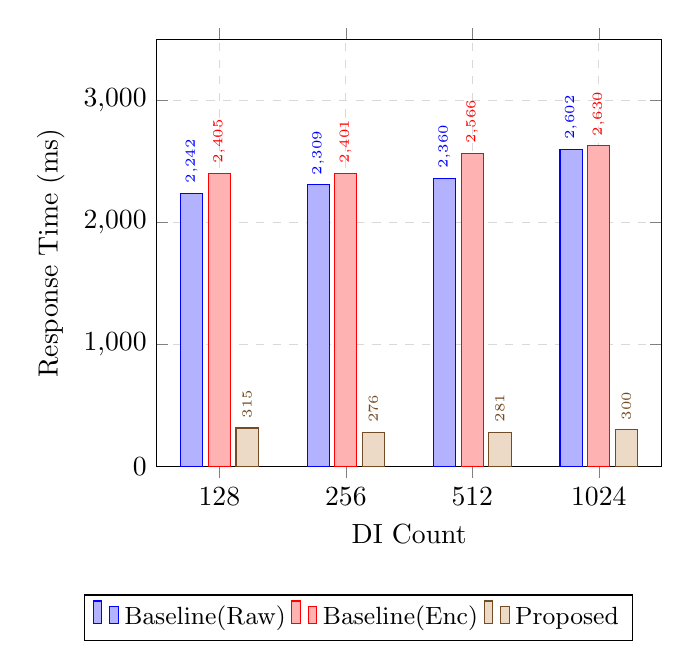
\begin{tikzpicture}
    \begin{axis}[
        ybar,
        enlarge x limits={abs=0.8cm},
        height=7cm,
        width=8cm,
        bar width=8pt,
        ylabel={Response Time (ms)},
        xlabel={DI Count},
        symbolic x coords={128, 256, 512, 1024},
        xtick=data,
        nodes near coords,
        nodes near coords style={rotate=90, anchor=west, font=\tiny, /pgf/number format/fixed},
        ymin=0,
        ymax=3500,
        legend style={at={(0.4,-0.3)}, anchor=north, legend columns=-1, font=\small},
        grid=major,
        grid style={dashed, gray!30},
    ]

    % Baseline (Raw)
    \addplot coordinates {(128, 2242) (256, 2309) (512, 2360) (1024, 2602)};
    
    % Baseline (Encrypted)
    \addplot coordinates {(128, 2405) (256, 2401) (512, 2566) (1024, 2630)};
    
    % Proposed
    \addplot coordinates {(128, 315) (256, 276) (512, 281) (1024, 300)};

    \legend{Baseline(Raw), Baseline(Enc), Proposed}
    \end{axis}
    \end{tikzpicture}
    \caption{average query response time for different DI count(single query, page size 30)}
\end{figure}

DI 수를 1024까지 늘려가며 측정한 응답 시간은 위와 같았다. 실시간 증명 생성이 없는 제안 모델은 모든 환경에서 압도적인 성능 차이(7, 8배)을 보여주었다. 앞서 벤치마크 실험에서 확인한 것 처럼, DI 수 증가에 따른 증명 생성 시간의 증가폭은 미미하였다. 따라서 이 실험에서도 baseline 모델의 전체 응답 시간의 변화는 DI 수의 증가폭에 비해 현저히 작은 것을 볼 수 있다. 또한 암호화 여부가 응답 시간에 미치는 영향은 최소 28ms(1024 DI)에서 최대 206ms(512 DI)에 불과했다. 이는 전체 응답 시간의 최대 0.09\%에 불과하다. 이처럼 데이터의 암호화 여부 역시 전체 응답 시간에서 차지하는 비율은 미미한 것을 볼 수 있다. 결국 응답 시간에 절대적인 영향을 미치는 것은 개별 증명 생성 시간이라는 것을 명백히 알 수 있다.

\begin{figure}[H]
    \centering
    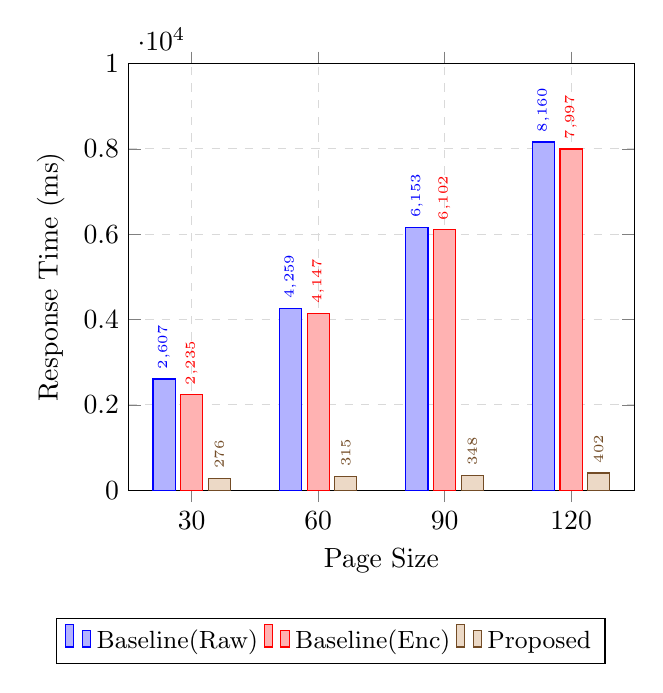
\begin{tikzpicture}
    \begin{axis}[
        ybar,
        enlarge x limits={abs=0.8cm},
        height=7cm,
        width=8cm,
        bar width=8pt,
        ylabel={Response Time (ms)},
        xlabel={Page Size},
        symbolic x coords={30, 60, 90, 120},
        xtick=data,
        nodes near coords,
        nodes near coords style={rotate=90, anchor=west, font=\tiny, /pgf/number format/fixed},
        ymin=0,
        ymax=10000,
        legend style={at={(0.4,-0.3)}, anchor=north, legend columns=-1, font=\small},
        grid=major,
        grid style={dashed, gray!30},
    ]

    % Baseline (Raw)
    \addplot coordinates {(30, 2607) (60, 4259) (90, 6153) (120, 8160)};
    
    % Baseline (Encrypted)
    \addplot coordinates {(30, 2235) (60, 4147) (90, 6102) (120, 7997)};
    
    % Proposed
    \addplot coordinates {(30, 276) (60, 315) (90, 348) (120, 402)};

    \legend{Baseline(Raw), Baseline(Enc), Proposed}
    \end{axis}
    \end{tikzpicture}
    \caption{average query response time for different page size(single query, 128 DI)}
\end{figure}

페이지 크기에 따른 응답 시간의 변화를 보면 이 점을 더욱 극명하게 확인할 수 있다. 페이지 크기를 늘린다는 것은 하나의 쿼리를 처리하는데 그만큼 더 많은 영지식 증명을 처리해야 한다는 의미이다. 위 그래프는 같은 환경에서 페이지 크기를 30에서 120까지 늘렸을 때의 응답 시간의 변화를 나타낸다. 페이지 크기가 커질 수록 baseline 모델은 증명 생성에 대한 부담이 선형적으로 증가하지만, 제안 모델은 그저 데이터베이스 조회 시간만 조금 늘어날 뿐이다. Baseline 모델은 페이지 크기가 30씩 증가할 때 마다 최소 30\%에서 최대 85\%까지도 응답시간이 증가한 반면, 제안 모델은 최소 10\%에서 최대 15\%가 증가하는 수준에 그쳤다. 이처럼 사전 생성된 증명을 채택한 제안 모델은 파라미터의 크기에 관계 없이 안정적인 확장성을 보여주고 있다.

\subsection{위협 모델 시뮬레이션 및 확장 보안에 대한 고찰}

\subsubsection{추론 공격 시뮬레이션 결과}

\begin{figure}[h]
    \centering
    \includegraphics[width=1\linewidth]{figure15-1.png}
    \includegraphics[width=1\linewidth]{figure15-2.png}
    \caption{Simulated adversary view}
\end{figure}

본 시스템의 취약점의 실질적인 위험을 평가하기 위해, 본 연구의 실험 데이터베이스가 모두 유출되었다는 가정하에 공격자 시점에서의 추론 공격(Inference Attack) 시뮬레이션을 수행하였다. 실험에 사용된 OWNERSHIP 테이블을 PROOF와 결합하여 각 DP가 가진 데이터들을 분류, 속성에 따라 각각의 그래프로 시각화 하였다. Figure 14는 특정 개인(DP)으로 부터 알아낼 수 있는 모든 정보를 시각화 한 결과이다. 공격자는 특정 DP가 소유한 모든 데이터의 종류, 수량과 범위의 분포을 알 수 있으며, 이에 기반해 개인에 대한 종합적인 건강 정보를 추론할 수 있다. 그래프에서 나타나듯, 공격자는 개별 튜플의 정확한 평문 수치를 알 수는 없으나, 붉은 선과 푸른 선 사이의 영역에 데이터 원문이 존재한다는 사실은 확인할 수 있다. 본 시스템에서 사용되는 범위 정보는 실제 의학적 참고 수치에 기반하였기 때문에, 이 정도 정보만으로도 해당 개인의 유병 내역(예: 당뇨, 고혈압 등)을 쉽게 예측할 수 있다. 

\bigskip

Figure 14의 실험결과를 해석하면 다음과 같다: 식별자 '0a3f578b-9230-4894-85ea-853b10505bcb'를 가진 개인(DP)은 30개의 속성에 대해 총 1066개의 데이터를 가지고 있었다. 이 중 공복혈당(Fasting Blood Sugar)은 0과 최대치 사이에 37개의 데이터가 분포해 있음을 알 수 있었다. 이 중 당뇨로 판정되는 125 이상의 데이터는 총 14개를 확인하였다. (참고로 해당 실험에 사용된 데이터셋은 난수에 기반해 생성되어 이같은 무작위적인 분포를 보였지만, 실제 데이터의 경우 훨씬 더 일관된 추세를 보일 것으로 예상된다.) 종합하면 공격자는 이 개인이 어떤 시점에 검진을 받았는지, 어떤 검사를 진행했는지, 그리고 데이터의 범위 분포 및 변화의 추이를 파악 할 수 있다. 나아가 이에 기반해 어떤 진단을 받았는지, 특정 시기의 건강 패턴이나 생활 습관이 어떻게 변화했는지 등을 추론해낼 수 있다. 여기에 전문적인 의학적 지식을 동원한다면 다른 속성 정보를 결합해 해당 개인에 대한 더 정확하고 종합적인 건강 정보를 추론해낼 수 있을 것이다.

\subsubsection{위협 완화 전략 및 트레이드오프}
이러한 구조적 위협을 완화하고 시스템을 고도화하기 위해, 본 연구는 다음과 같은 추가적인 보안 전략의 적용을 제안한다.

\bigskip

첫째, 더미 데이터 주입을 통한 교란이다. DI 혹은 DP측에서 최초로 증명을 생성할 때, 실제 데이터와 다른 범위에 속하는 데이터를 생성, 이에 대한 더미 증명을 생성한다. 이처럼 모든 증명에 대해, 수학적으로는 참이지만 실존하지는 않는 거짓 양성(false positive) 증명을 1대 1로 생성하여 SS에 전달한다. 여기서 어느 쪽이 진짜 증명인지는 오직 이를 생성한 DI 혹은 DP만이 알고 있으며, SS 조차도 이를 알 수 없다. 데이터 수요자(DC)는 데이터 구매 결정 후 소유자로부터 데이터 원문을 넘겨받는 시점에서 진짜 증명을 구분할 수 있게 한다. 이 경우 공격자가 소유권 정보를 탈취하여 분석하더라도, 가짜 증명으로 발생한 노이즈로 인해 특정 개인의 병력을 확정적으로 추론하는 것이 불가능해진다. 다만 이러한 구조는 공격자 뿐만 아니라 수요자의 검색 결과에게도 노이즈를 추가하게 되므로 구매 과정에서 이를 효율적으로 필터링 해내는 추가적인 시스템이 요구된다.

\bigskip

둘째, 비공모 다중 서버(Non-colluding Multi-server) 기반의 비밀 분산(Secret Sharing)이다. 검색 서버를 서로 공모하지 않는 두 개 이상의 독립된 서버로 분리하고, OWNERSHIP 테이블의 식별자 정보를 안전한 다자간 컴퓨팅(MPC) 프로토콜을 통해서만 연산되도록 분산 저장하는 방식이다. 이는 현실적으로 적용 가능한 가장 안정적인 방법이며, 더미 데이터 주입과 달리 데이터 수요자 측에 부담을 주지 않는다는 장점이 있다. 공격자는 특정 임계값을 넘는 숫자의 서버를 해킹하지 않는 이상 복호화 키를 복원할 수 없으며, 이를 통해 단일 서버가 장악되더라도 소유권 정보가 복원되지 않는 강력한 기밀성을 확보할 수 있다. 단, 이는 SS 측의 연산 오버헤드를 크게 증가시키는 방법이며, MPC 프로토콜이 검색의 실시간성에 끼치는 영향은 별도의 실험이 필요할 것이다.

\bigskip

결론적으로, 현재 상황에서 본 시스템이 지닌 보안 취약점을 완벽히 보완할 방법은 없어보인다. 어떤 방법을 선택하더라도 사용자 편의성의 희생, 검색의 실시간성의 손실 혹은 연산 비용의 증가는 필수 불가결한 부작용으로 판단된다. 따라서 본 연구는 대규모 데이터 검색의 실시간성과 실용성을 달성하기 위해 OWNERSHIP 테이블 유지라는 전략적 타협을 선택하였다. 향후 위에서 제시한 더미 주입 및 다중 서버 기반의 비밀 분산 기법 등을 발전시킴으로써 부작용은 최소화 하며 최악의 보안 위협까지 완벽히 방어할 수 있는 범용적인 시스템으로 확장할 수 있기를 기대한다.


\clearpage
\section{결론}
%! TEX root = main.tex

본 연구는 민감한 수치형 의료 데이터의 프라이버시를 완벽히 보호하면서도 실시간 검색을 가능하게 하는 영지식 증명(zk-SNARK) 기반의 새로운 사전 증명 검색 시스템을 제안하고 그 실효성을 입증하였다. 기존의 암호화 데이터베이스 연구들은 일부 정보 노출을 허용하여 보안성이 훼손되거나(OPE 등), 완전한 은닉을 추구하다가 실용성을 상실하는(ZKSQL 등) '데이터 프라이버시와 검색의 이중성(Dichotomy)'이라는 근본적인 딜레마에 빠져 있었다. 본 연구는 데이터의 원문을 서버에 일절 저장하지 않고 '사전 정의된 임상 참고치'에 대한 범위 증명 객체만을 저장하는 방식을 도입함으로써 이 문제를 성공적으로 타파하였다.

\subsection{연구의 의의}
본 연구의 가장 큰 학술적, 실용적 의의는 다음과 같다. 첫째, 기존 검증 가능한 데이터베이스 시스템의 치명적 한계였던 실시간 증명 연산 병목 현상을 완벽히 제거하였다. 설계 방식 비교 실험을 통해 제안 시스템이 응답 반환 개수(K)에 비례하여 선형적으로 지연되는 기존 모델의 한계(O(K))를 극복하고, 순수 데이터베이스 I/O 시간에 수렴하는 O(1) 스케일의 압도적인 검색 속도를 달성함을 확인하였다. 둘째, 다중 쿼리(Composite Query) 처리 시 필연적으로 발생하는 '소유권 증명' 문제를 단일 그룹 커밋과 실시간 증명의 일괄 생성을 통해 해결하였다. 이를 통해 다수의 서브 쿼리를 처리할 때도 암호학적 연산 지연을 500ms 미만으로 통제하였으며, 네트워크 부하 역시 약 4.9KB 수준으로 최소화하여 상용 클라우드 서비스 환경에서도 충분히 도입 가능한 수준의 실용성을 확보하였다.

\subsection{연구의 한계} 
그러나 본 연구는 대규모 검색 시스템으로서의 '실시간성'을 달성하기 위해 몇 가지 의도된 시스템적 절충을 채택하였으며, 이는 다음과 같은 한계점을 지닌다. 첫째, 다중 쿼리 결과의 실시간 그룹화를 위해 검색 서버(SS) 내부에 외부와 격리된 OWNERSHIP 매핑 테이블을 유지하였다. 비록 원문 데이터는 영지식 증명 뒤에 안전하게 은닉되지만, 서버가 완전히 장악당하는 최악의 시나리오에서는 특정 소유자의 데이터 분포 정보가 노출될 수 있는 위험이 존재한다. 둘째, 본 시스템은 서버를 '반신뢰(Semi-honest) 주체'로 가정하였다. 결과에 포함된 데이터들이 조작되지 않았음(Soundness)은 수학적으로 완벽히 증명하지만, 악의적인 서버가 조건에 부합하는 결과를 고의로 누락하는 행위(Incompleteness)를 원천적으로 검증하거나 방어하지는 못한다. 이는 완전한 은닉성 하에서 무결성을 검증하기 위해 막대한 통신 및 연산 오버헤드를 유발하는 기존 연구들의 한계를 피하기 위한 불가피한 선택이었다.

\subsection{향후 과제}
본 연구의 한계를 보완하고 시스템의 범용성을 넓히기 위해 다음과 같은 후속 연구를 제안한다. 첫째, 악의적 위협 모델 하에서도 검색의 실시간성을 크게 훼손하지 않으며 쿼리 결과의 누락 없음(Completeness)을 증명할 수 있는 고도화된 검증 프로토콜에 대한 연구가 필요하다. 둘째, 현재 시스템은 사전 정의된 이산적인 구간(Pre-defined Range) 정보에 기반하고 있다. 향후에는 동형 암호나 다자간 컴퓨팅(MPC) 등의 최신 암호학적 원형들을 영지식 증명과 결합하여, 연속적인 범위 검색이나 텍스트와 같은 비수치형 데이터에 대해서도 온디맨드(On-demand)로 실시간 증명이 가능한 범용적인 프라이버시 보존 검색 아키텍처로 발전시켜 나갈 계획이다.

\clearpage
\bibliographystyle{plain}
\bibliography{reference}

%! TEX root = main.tex

\clearpage

{\noindent \bfseries Abstract \par}
\vspace{1cm}
Since the emergence of generative AI services, academia and industry worldwide have begun to demand massive amounts of data for model training. As the demand for high-quality data in various fields has surged to unprecedented levels, data has attained a status akin to a strategic asset. Consequently, platform companies that previously monopolized data in their respective fields have exerted immense influence. Meanwhile, the individuals who contributed to the creation of that data have received no compensation and continue to rely on the untrustworthy infrastructure of corporations. Web 3.0 has begun to receive spotlight as a vision to correct ownership structures in this era of data assets, and many engineers have focused on technological development for this purpose. In particular, numerous studies have aimed to implement systems that allow for the free and safe trading of data while protecting the ownership of the original data author. As part of such an effort, this study proposes a system that uses zero-knowledge proof technology to search for 'evidence' rather than the original raw data. Specifically, by proposing a system that can search for numerical medical data based on ranges, individual patients can upload evidence to a platform without fear of their medical data being leaked. Data consumers can then search for this evidence to verify the existence of data that fits their required range. By storing only zk-SNARK-based zero-knowledge proof data on a centralized server, this system eliminates the risk of personal information leakage while simultaneously providing an efficient search mechanism for the data ranges desired by consumers. \\ \\

{\noindent \bfseries Keywords \par}
\noindent data privacy, zero knowledge proof, data exchange platform, zk-SNARK, medical data, range proof


\end{document}
